\documentclass[aspectratio=1610]{beamer}
\usepackage[utf8]{inputenc}
\usepackage{ragged2e}
\usepackage{xcolor}
\usepackage[italian]{babel}
\usepackage{multirow}
\usepackage{silence}
\WarningFilter{beamer}{}
\WarningFilter{metropolis}{}
\usetheme[progressbar=frametitle,titleformat=smallcaps]{metropolis}
\setbeamertemplate{frame numbering}[fraction]
\setbeamercovered{dynamic}
\definecolor{rosso}{RGB}{255, 0, 0}
\definecolor{giallo}{RGB}{254,212,23}
\hypersetup{colorlinks=true,linkcolor=black,urlcolor=rosso}
\setbeamercolor{palette primary}{fg=black, bg=giallo}
\setbeamercolor{background canvas}{bg=white}
\setbeamercolor{normal text}{fg=black}
\setbeamercolor{progress bar}{fg=rosso}
\setbeamercolor{framesubtitle}{fg=rosso}
\setbeamercolor{normal text .dimmed}{fg=giallo}
\setbeamercolor{block title alerted}{fg=rosso, bg=giallo}
\setbeamerfont{caption}{size=\tiny}
\setbeamerfont{caption name}{size=\tiny}
\setlength{\abovecaptionskip}{0pt}
\makeatletter
\metroset{block=fill}
\setlength{\metropolis@progressinheadfoot@linewidth}{1pt} 
\setlength{\metropolis@progressonsectionpage@linewidth}{1pt}
\setlength{\metropolis@titleseparator@linewidth}{1pt}
\makeatother

\title{Cloud e SaaS per le PMI}
\subtitle{Selezione, configurazione e governance degli 
strumenti in abbonamento}
\date{}
\institute{\textit{
        Fonti:
        \begin{itemize}
            \item[-] \href{https://www.zanichelli.it/ricerca/prodotti/system-afm-amministrazione-finanza-marketing-informatica-per-istituti-tecnici-economici-lorenzi}{System: Amminitrazione Finanza e Marketing, Informatica per Istituti Tecnici Economici}
            \item[-] \href{https://it.wikipedia.org/wiki/Software_as_a_service}{Wikipedia: Software as a Service}
            \item[-] \href{https://www.odoo.com/it_IT}{Software gestionale in cloud: Odoo}
        \end{itemize}
    }
}
\author{Gabriele Alessandro Cazzaniga}

\begin{document}

\begin{frame}[plain, noframenumbering]
    \titlepage
\end{frame}

\section{Contestualizzazione e inquadramento}

\begin{frame}{Contestualizzazione e inquadramento}
    \begin{alertblock}{Contestualizzazione}
        \begin{minipage}{0.98\linewidth}
            \justifying
            Istituto Tecnico Economico - Indirizzo \textbf{Amministrazione Finanza e Marketing} \\
            (art. \textbf{Sistemi Informativi Aziendali}).
            \bigskip
            \begin{itemize}
                \item \textbf{Tipologia lezione}: Lezione iniziale
                \item \textbf{Disciplina}: Informatica
                \item \textbf{Classe}: IV
                \item \textbf{Ore/settimana}: 5
            \end{itemize}
            \bigskip      
        \end{minipage}
    \end{alertblock}
\end{frame}

\begin{frame}{Contestualizzazione e inquadramento}
    \begin{alertblock}{Contestualizzazione}
        \begin{minipage}{0.98\linewidth}
            \justifying
            La classe è composta da 24 studenti, di cui \textbf{12 maschi} e \textbf{12 femmine}. \\
            All'interno del gruppo classe sono presenti \textbf{2 studenti certificati con BES} per disturbi 
            dell'apprendimento:
            \bigskip
            \begin{itemize}
                \item \textbf{1} studentessa certificata con DSA per dislessia;
                \item \textbf{1} studente con difficoltà socio-economiche certificate.
            \end{itemize}
            \bigskip      
        \end{minipage}
    \end{alertblock}
\end{frame}

\begin{frame}{Inquadramento}
    \begin{figure}
        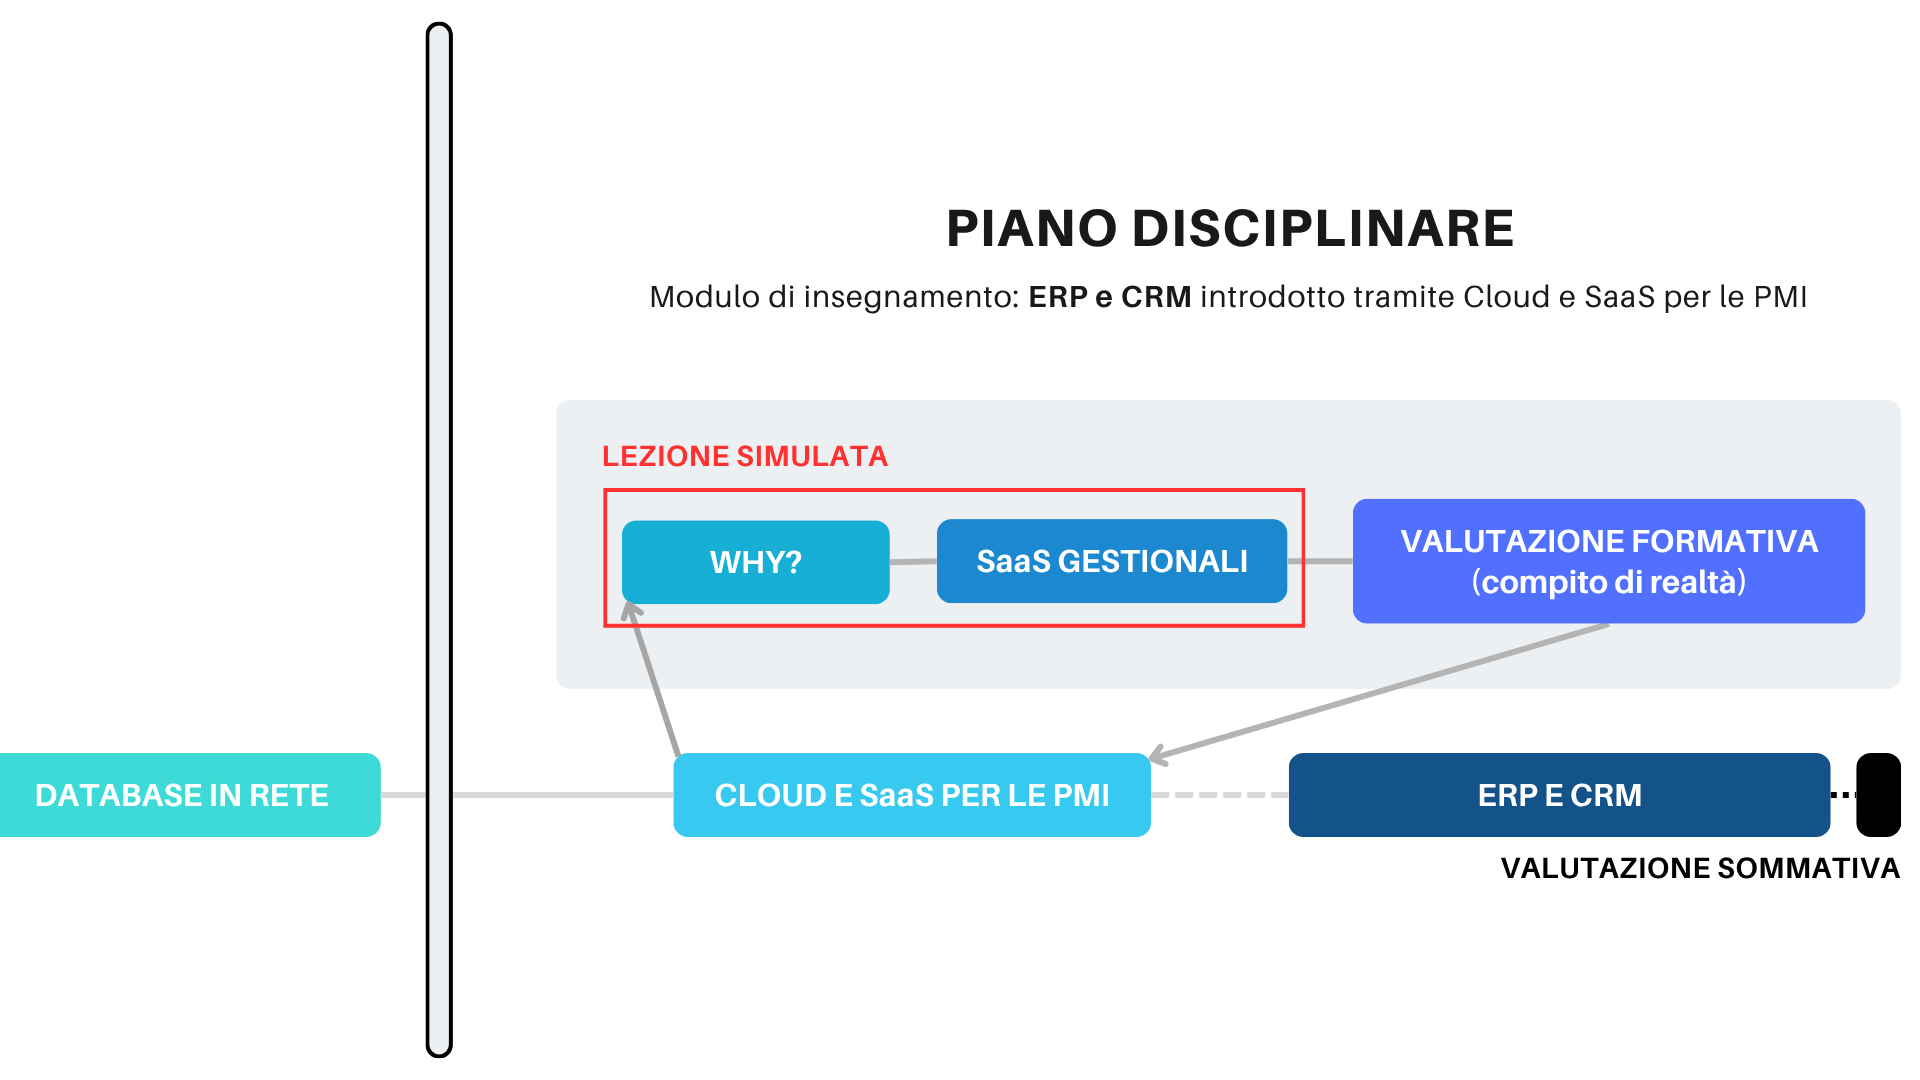
\includegraphics[width=\linewidth]{pianodisciplinare.png}
        \caption{{creata con \href{https://www.canva.com/}{Canva}}}
    \end{figure}
\end{frame}


\section{Prerequisiti e obiettivi}

\begin{frame}{Prerequisiti}
    \begin{alertblock}{Prerequisiti}
        \begin{minipage}{0.98\linewidth}
            \justifying
            \begin{itemize}
                \item \textbf{Reti informatiche}: Cloud Computing e funzionamento base di Internet.
                \item \textbf{Sistemi Informativi Aziendali}: concetti di base sui software gestionali.
            \end{itemize}
        \end{minipage}
    \end{alertblock}
\end{frame}

\begin{frame}{Obiettivo Lezione simulata}
    \begin{minipage}{0.98\linewidth}
        \centering
        Obiettivo specifico della lezione simulata:\\
        \huge
        \textit{``Introdurre gli studenti ai criteri di scelta e gestione 
        dei principali software gestionali erogati in cloud.''}\\
    \end{minipage}\\
    \bigskip
\end{frame}

\begin{frame}{Obiettivi - Competenze}
    \begin{figure}
        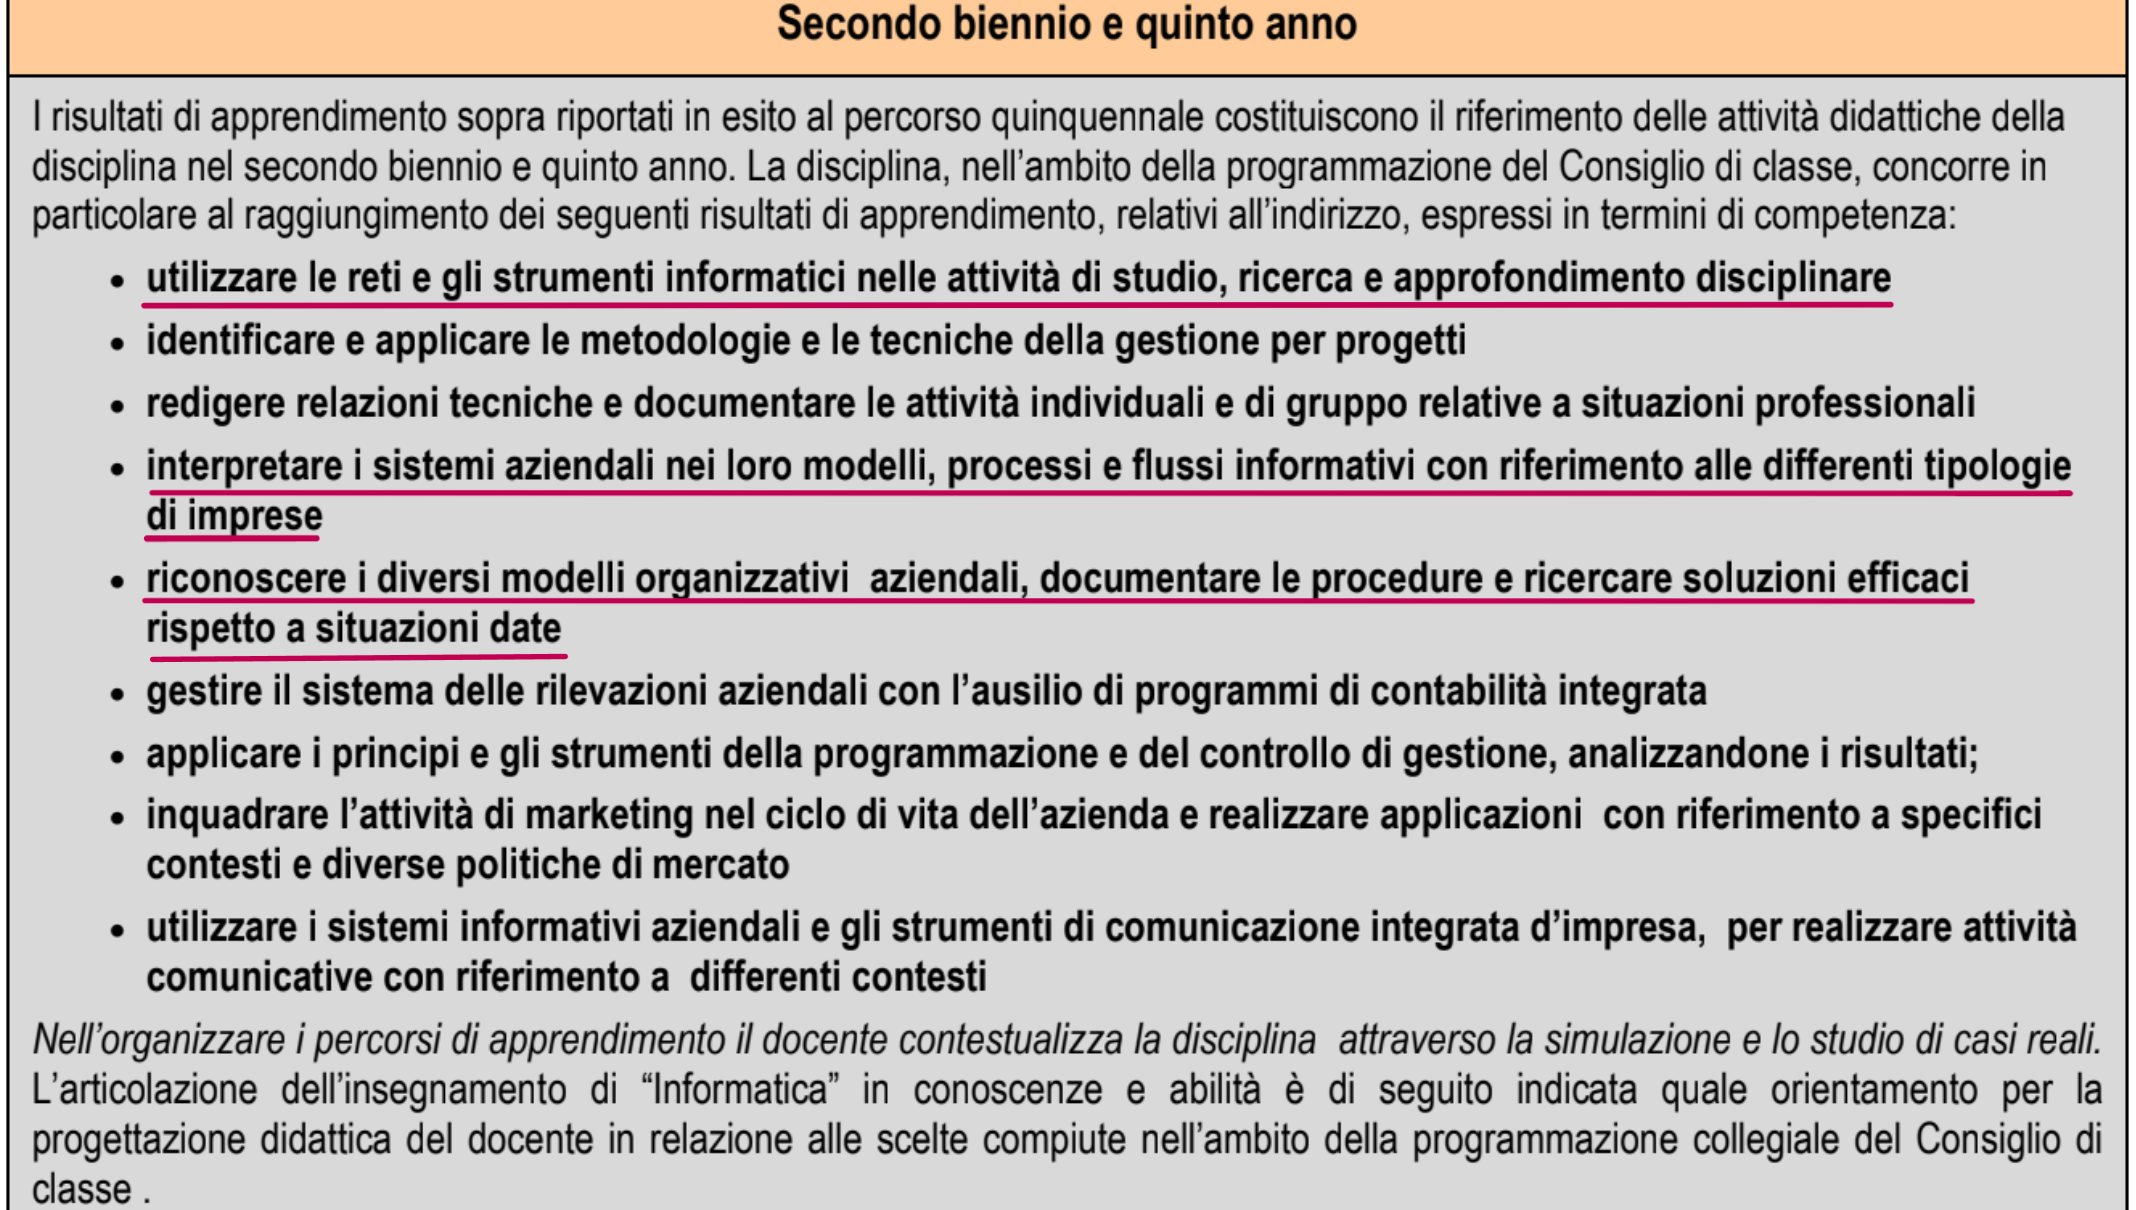
\includegraphics[width=\linewidth]{competenze.png}
        \caption{{fonte: \href{https://sanoma.it/newsletter-disciplinari/paramondonline/programmi-ministeriali-istituti-tecnici}{Linee guida ministeriali: AFM art. SIA }}}
    \end{figure}
\end{frame}

\begin{frame}{Obiettivi - Abilità e Conoscenze}
    \begin{figure}
        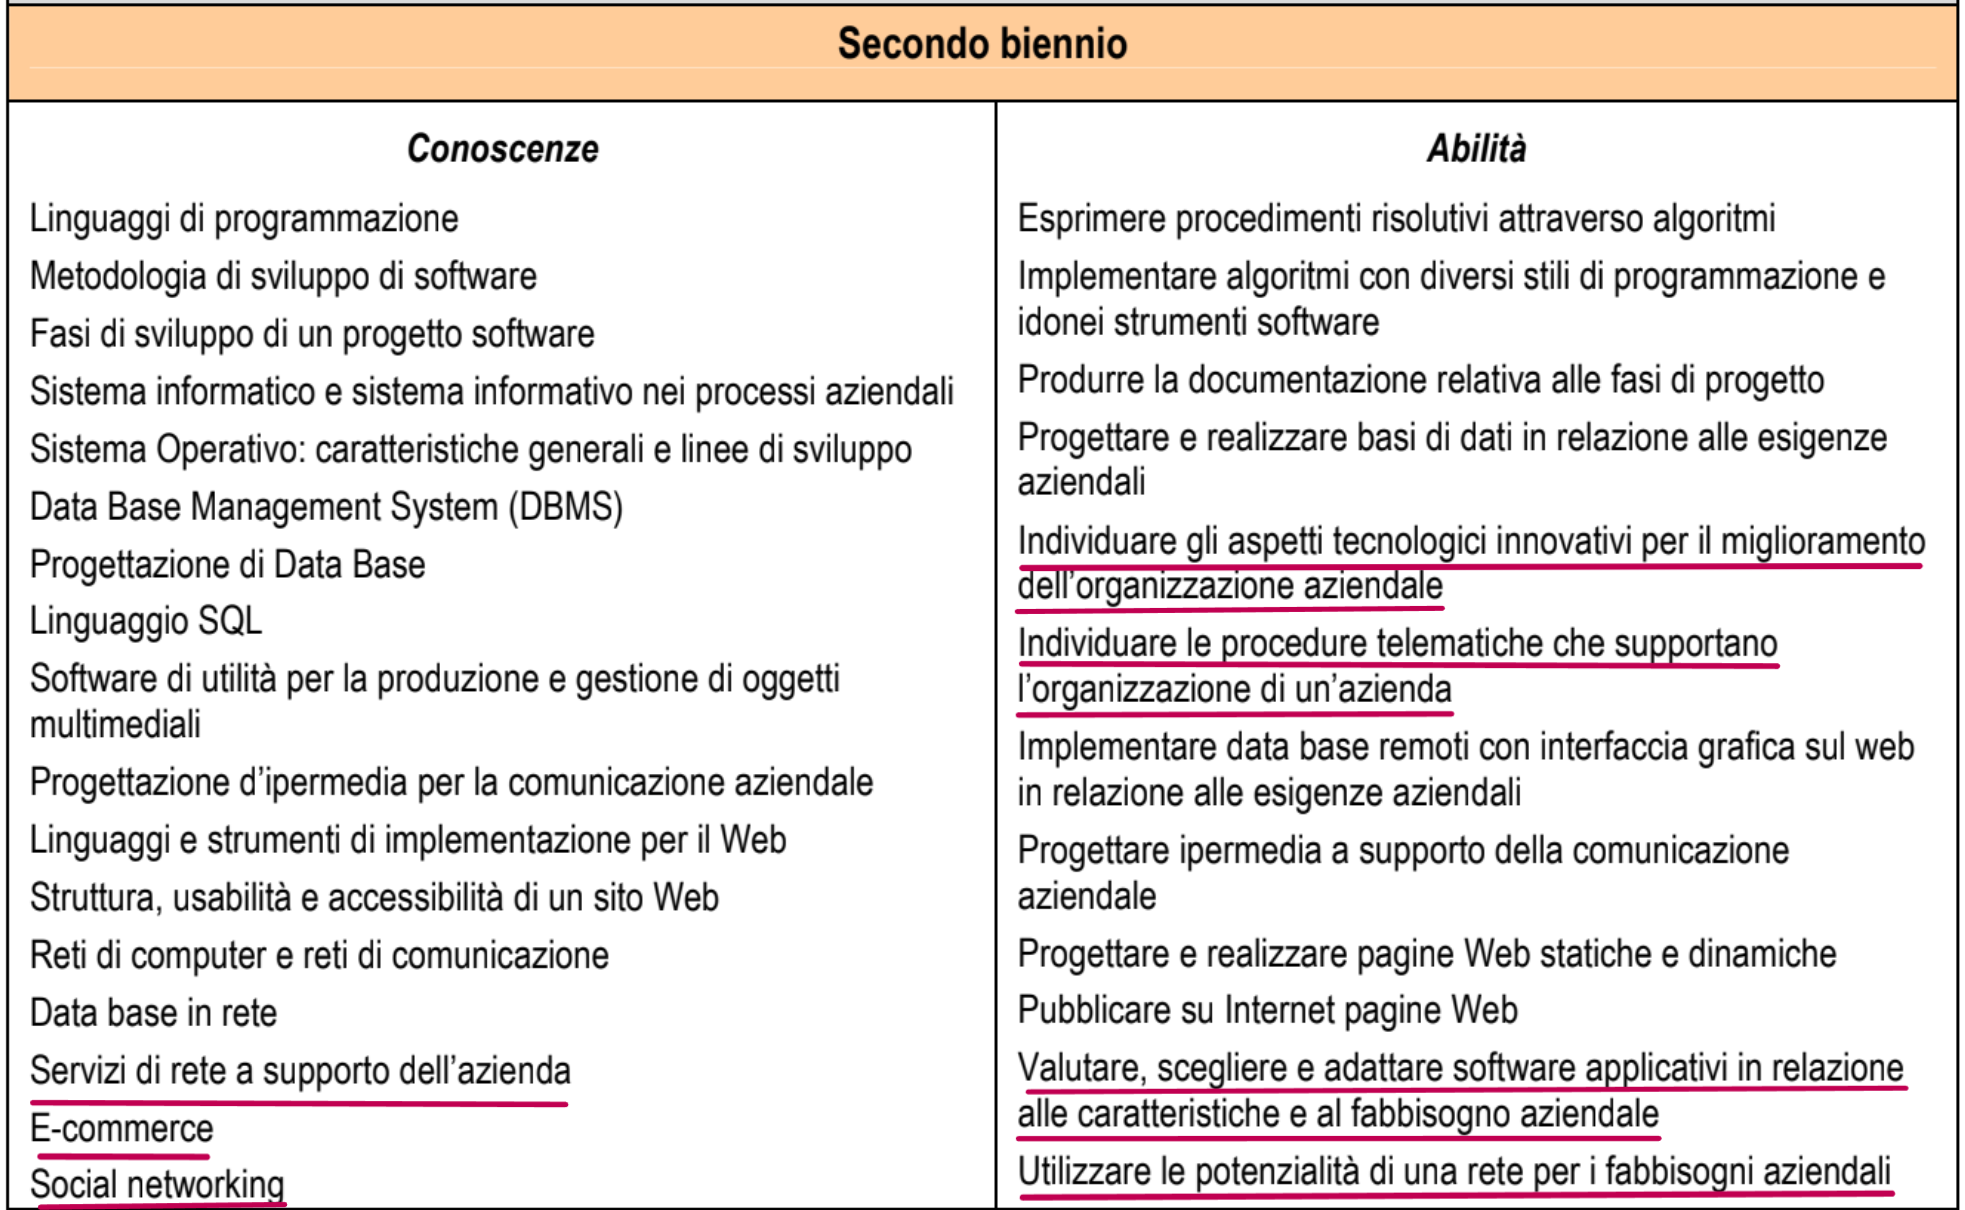
\includegraphics[width=.9\linewidth]{abilitaconoscenze.png}
        \caption{{fonte: \href{https://sanoma.it/newsletter-disciplinari/paramondonline/programmi-ministeriali-istituti-tecnici}{Linee guida ministeriali: AFM art. SIA }}}
    \end{figure}
\end{frame}

\section{Metodologie e strumenti}

\begin{frame}{Metodologie e strumenti}
    \begin{alertblock}{Metodologie}
        \begin{minipage}{0.98\linewidth}
            \justifying
            \begin{itemize}
                \item \textbf{Lezione partecipata}: coinvolgimento attivo degli studenti durante la lezione;
                \item \textcolor<3>{red}{\textbf{Cooperative learning}}: attività di gruppo per favorire l'apprendimento collaborativo;
                \item \textcolor<3>{red}{\textbf{Learning by doing}}: apprendimento attraverso l'esperienza pratica.
            \end{itemize}
            \bigskip
        \end{minipage}
    \end{alertblock}
    \pause
    \begin{alertblock}{Strumenti}
        \begin{minipage}{0.98\linewidth}
            \justifying
            \begin{itemize}
                \item \textcolor<3>{red}{\textbf{Computer}}: \textcolor<3>{red}{forniti dalla scuola}, con accesso a Internet;
                \item \textbf{Software gestionale in cloud}: Odoo (\textcolor<3>{red}{versione gratuita});
                \item \textbf{Materiale didattico}: slide consultabili online e \textcolor<3>{red}{handout cartacei};
                \item \textbf{Piattaforma per la consegna degli elaborati}: Google suite.
            \end{itemize}
            \bigskip
            \pause
            \tiny{\textbf{Strumenti BES}}\\
            \tiny{\textcolor<3>{red}{In rosso sono evidenziate le misure compensative per gli studenti con BES (dislessia, difficoltà socio-economiche).}}
        \end{minipage}
    \end{alertblock}
\end{frame}

\section{Lezione simulata}

\begin{frame}[plain, noframenumbering]
    \titlepage
\end{frame}

\begin{frame}{WHY?}
    \only<1 | handout:1>{\begin{figure}
        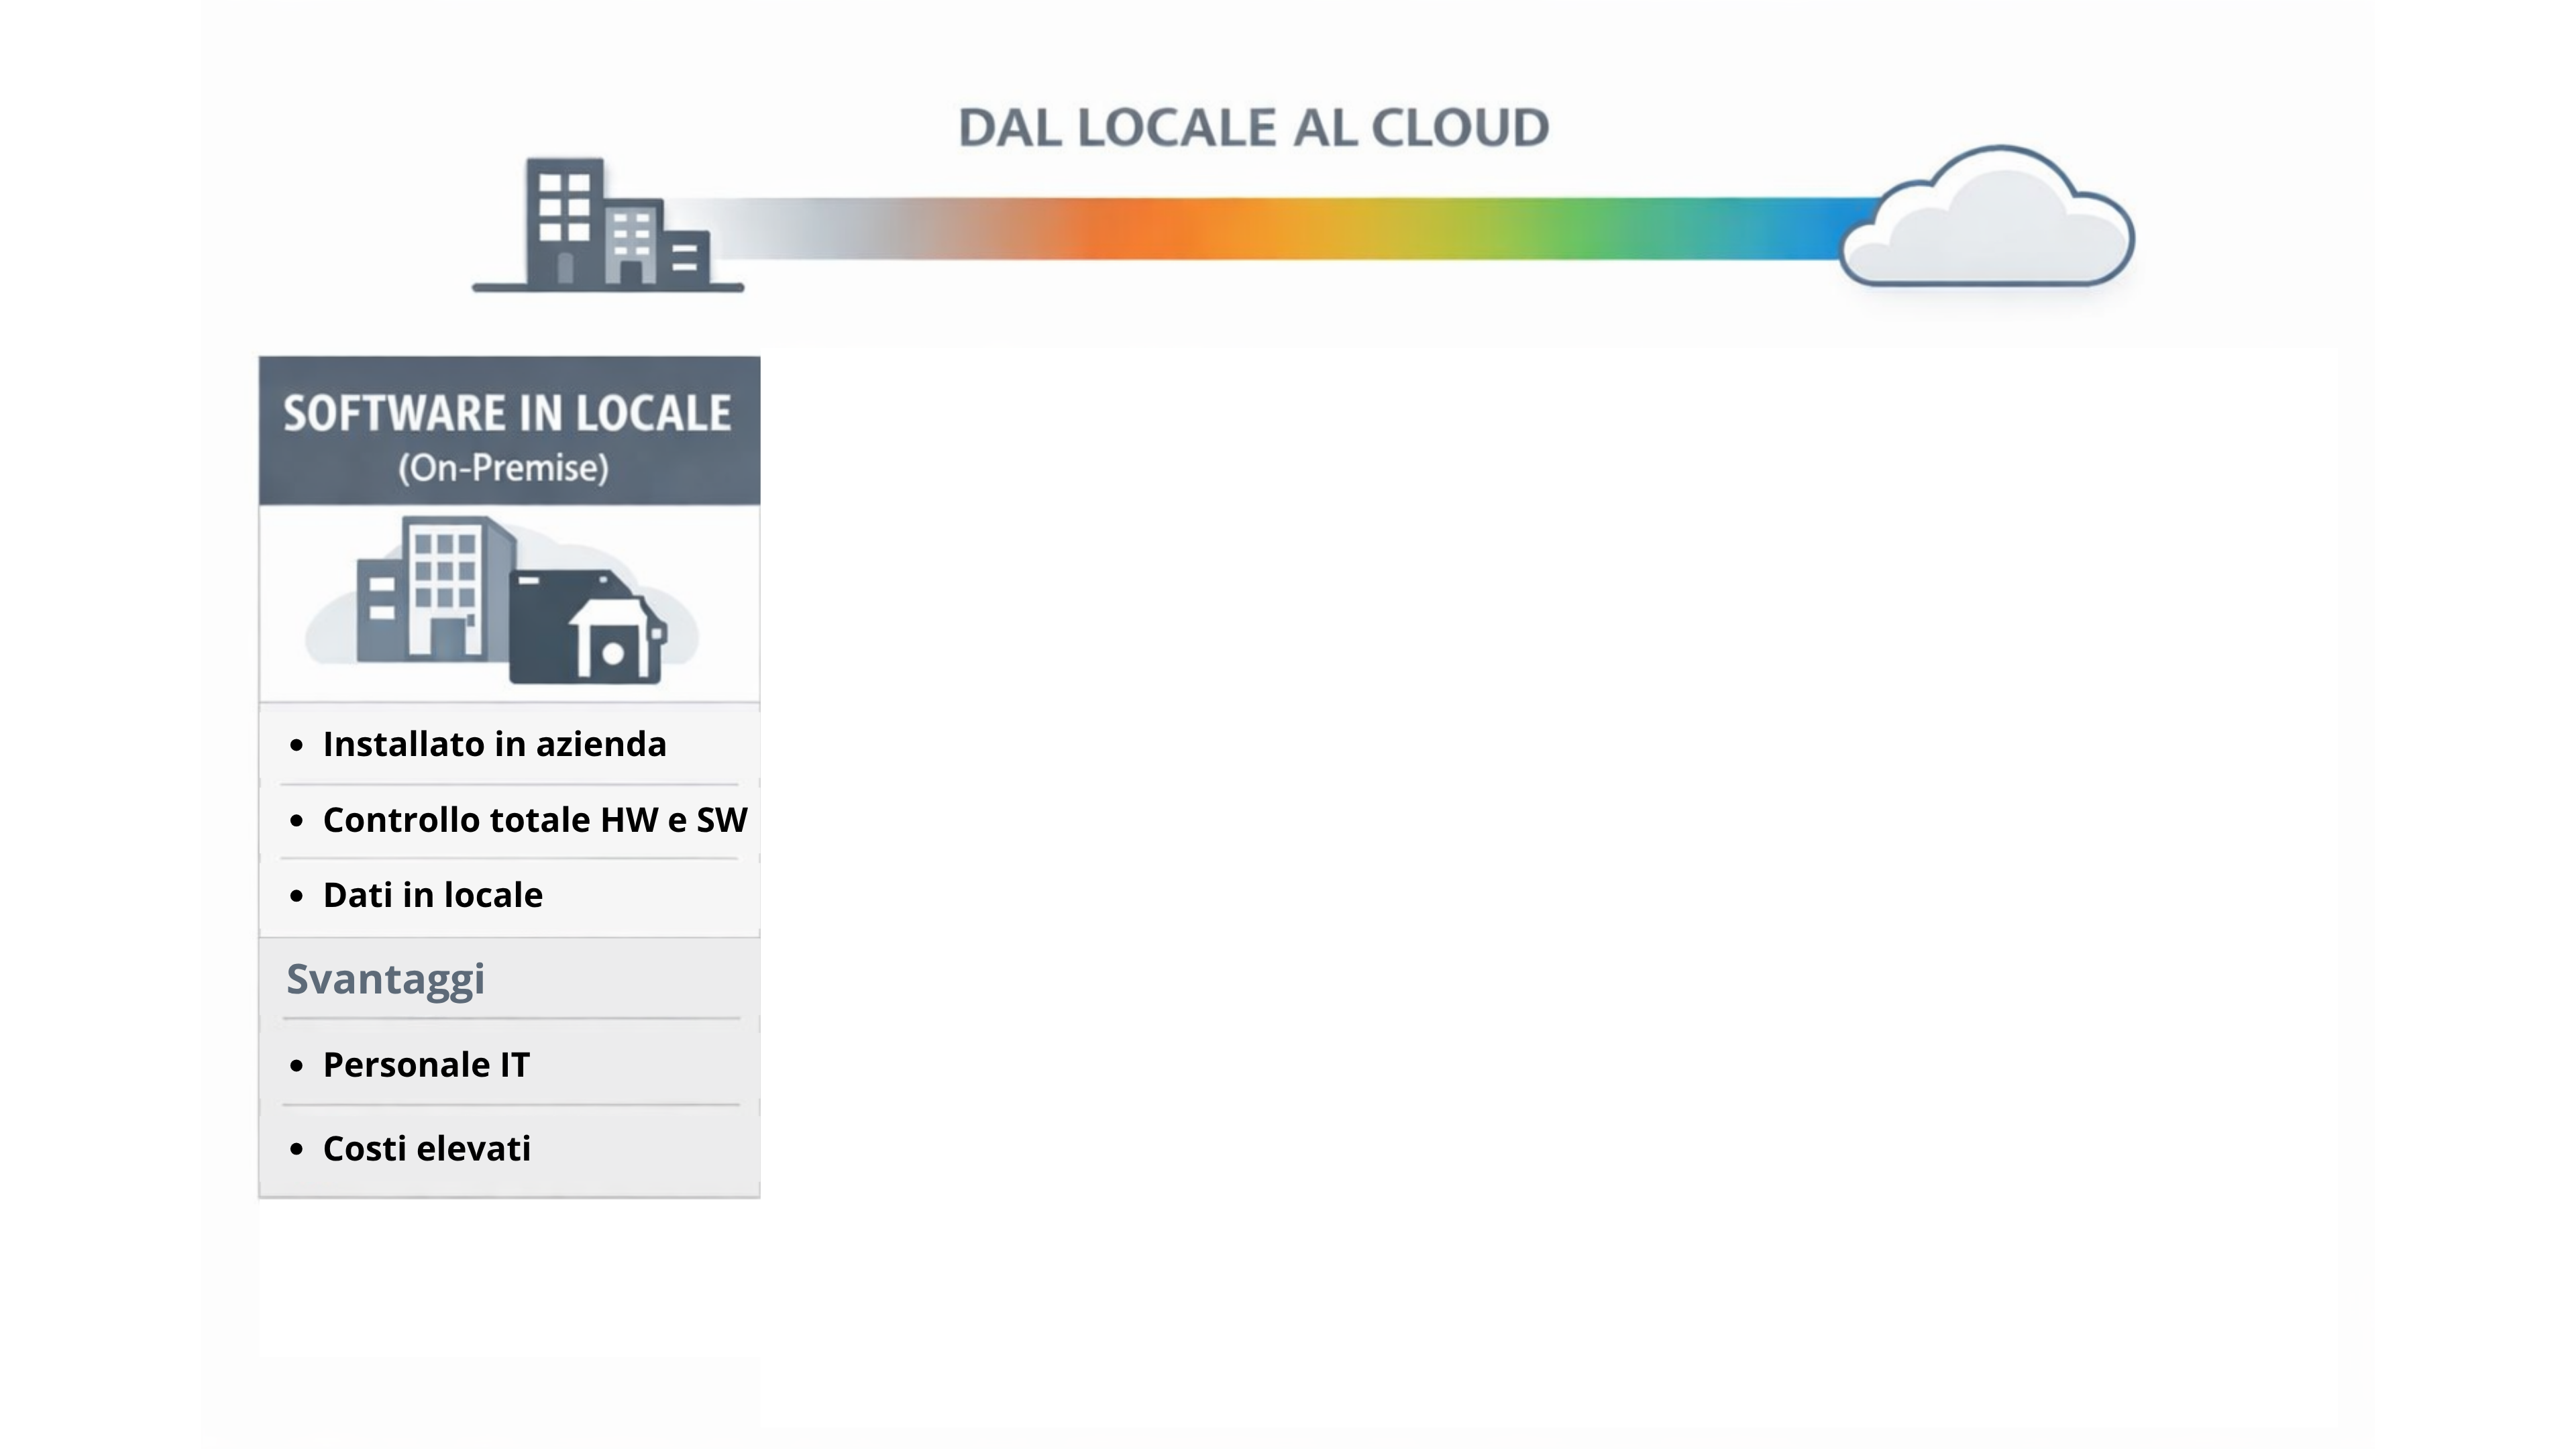
\includegraphics[width=\linewidth]{confronto1.png}
        \caption{{creata con \href{https://copilot.microsoft.com/}{Copilot}} e modificata con \href{https://www.canva.com/}{Canva}}
    \end{figure}}
    \only<2 | handout:2>{\begin{figure}
        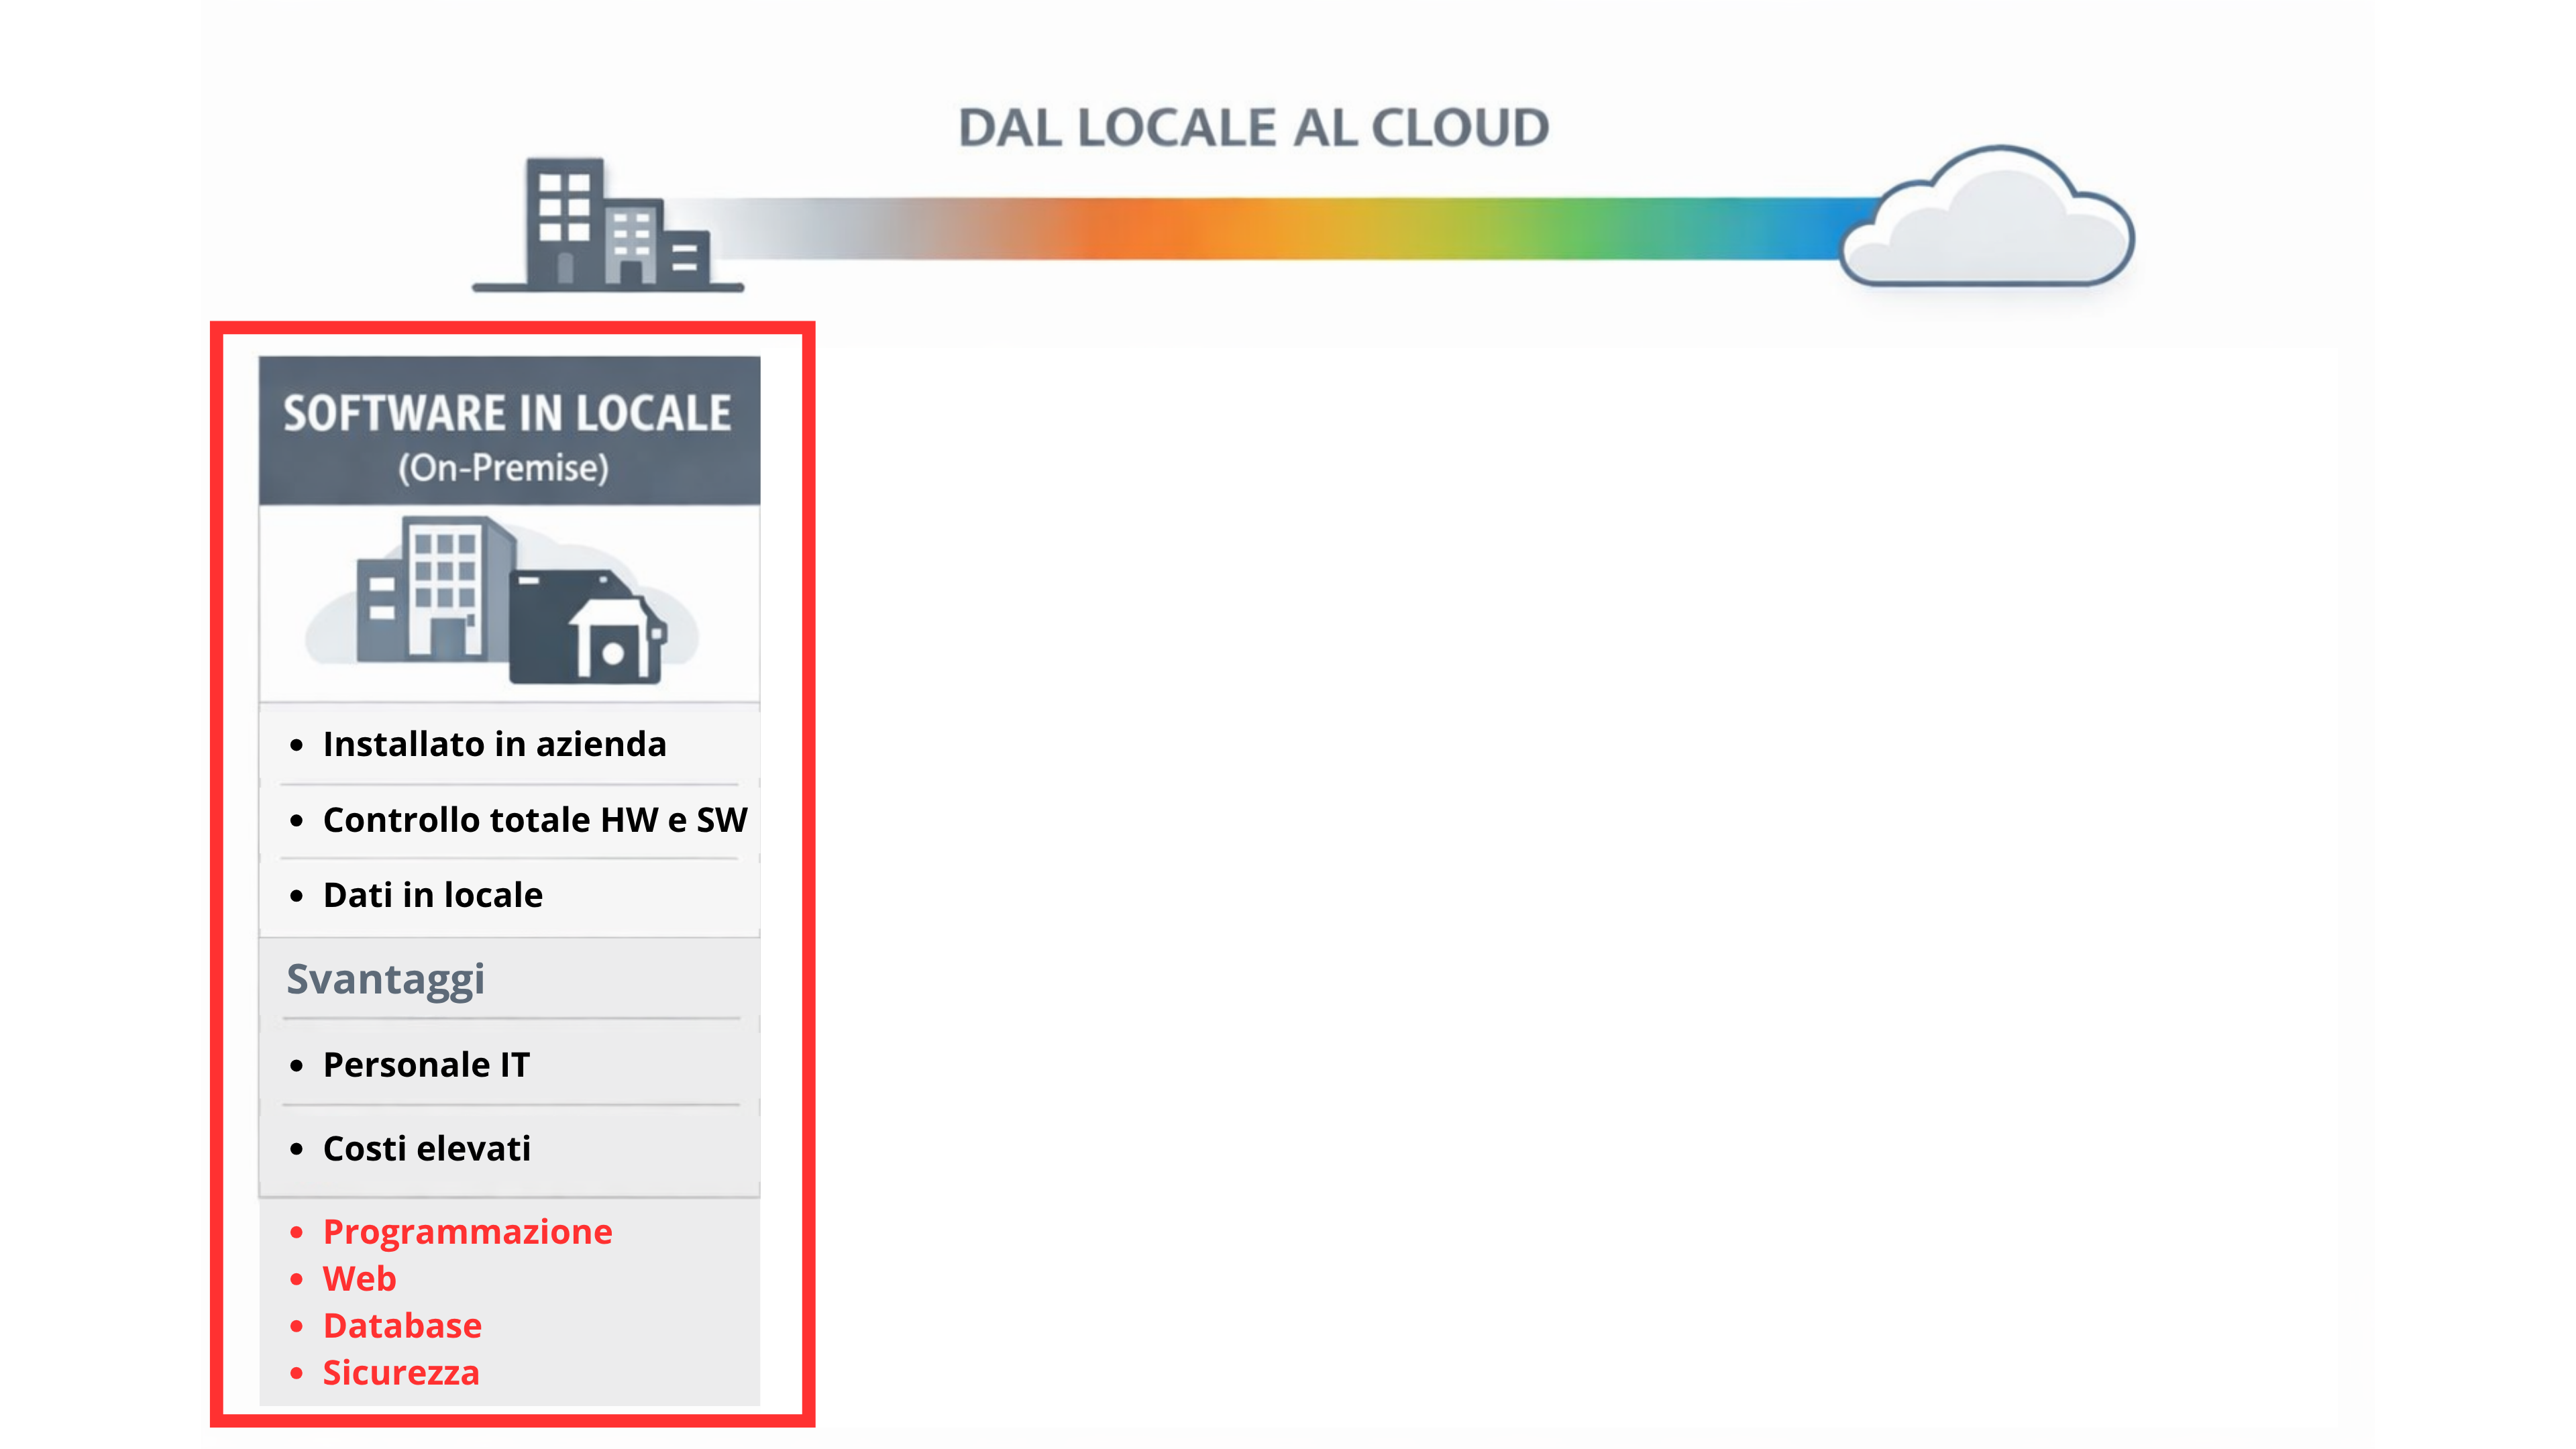
\includegraphics[width=\linewidth]{confronto2.png}
        \caption{{creata con \href{https://copilot.microsoft.com/}{Copilot}} e modificata con \href{https://www.canva.com/}{Canva}}
    \end{figure}}
    \only<3 | handout:3>{\begin{figure}
        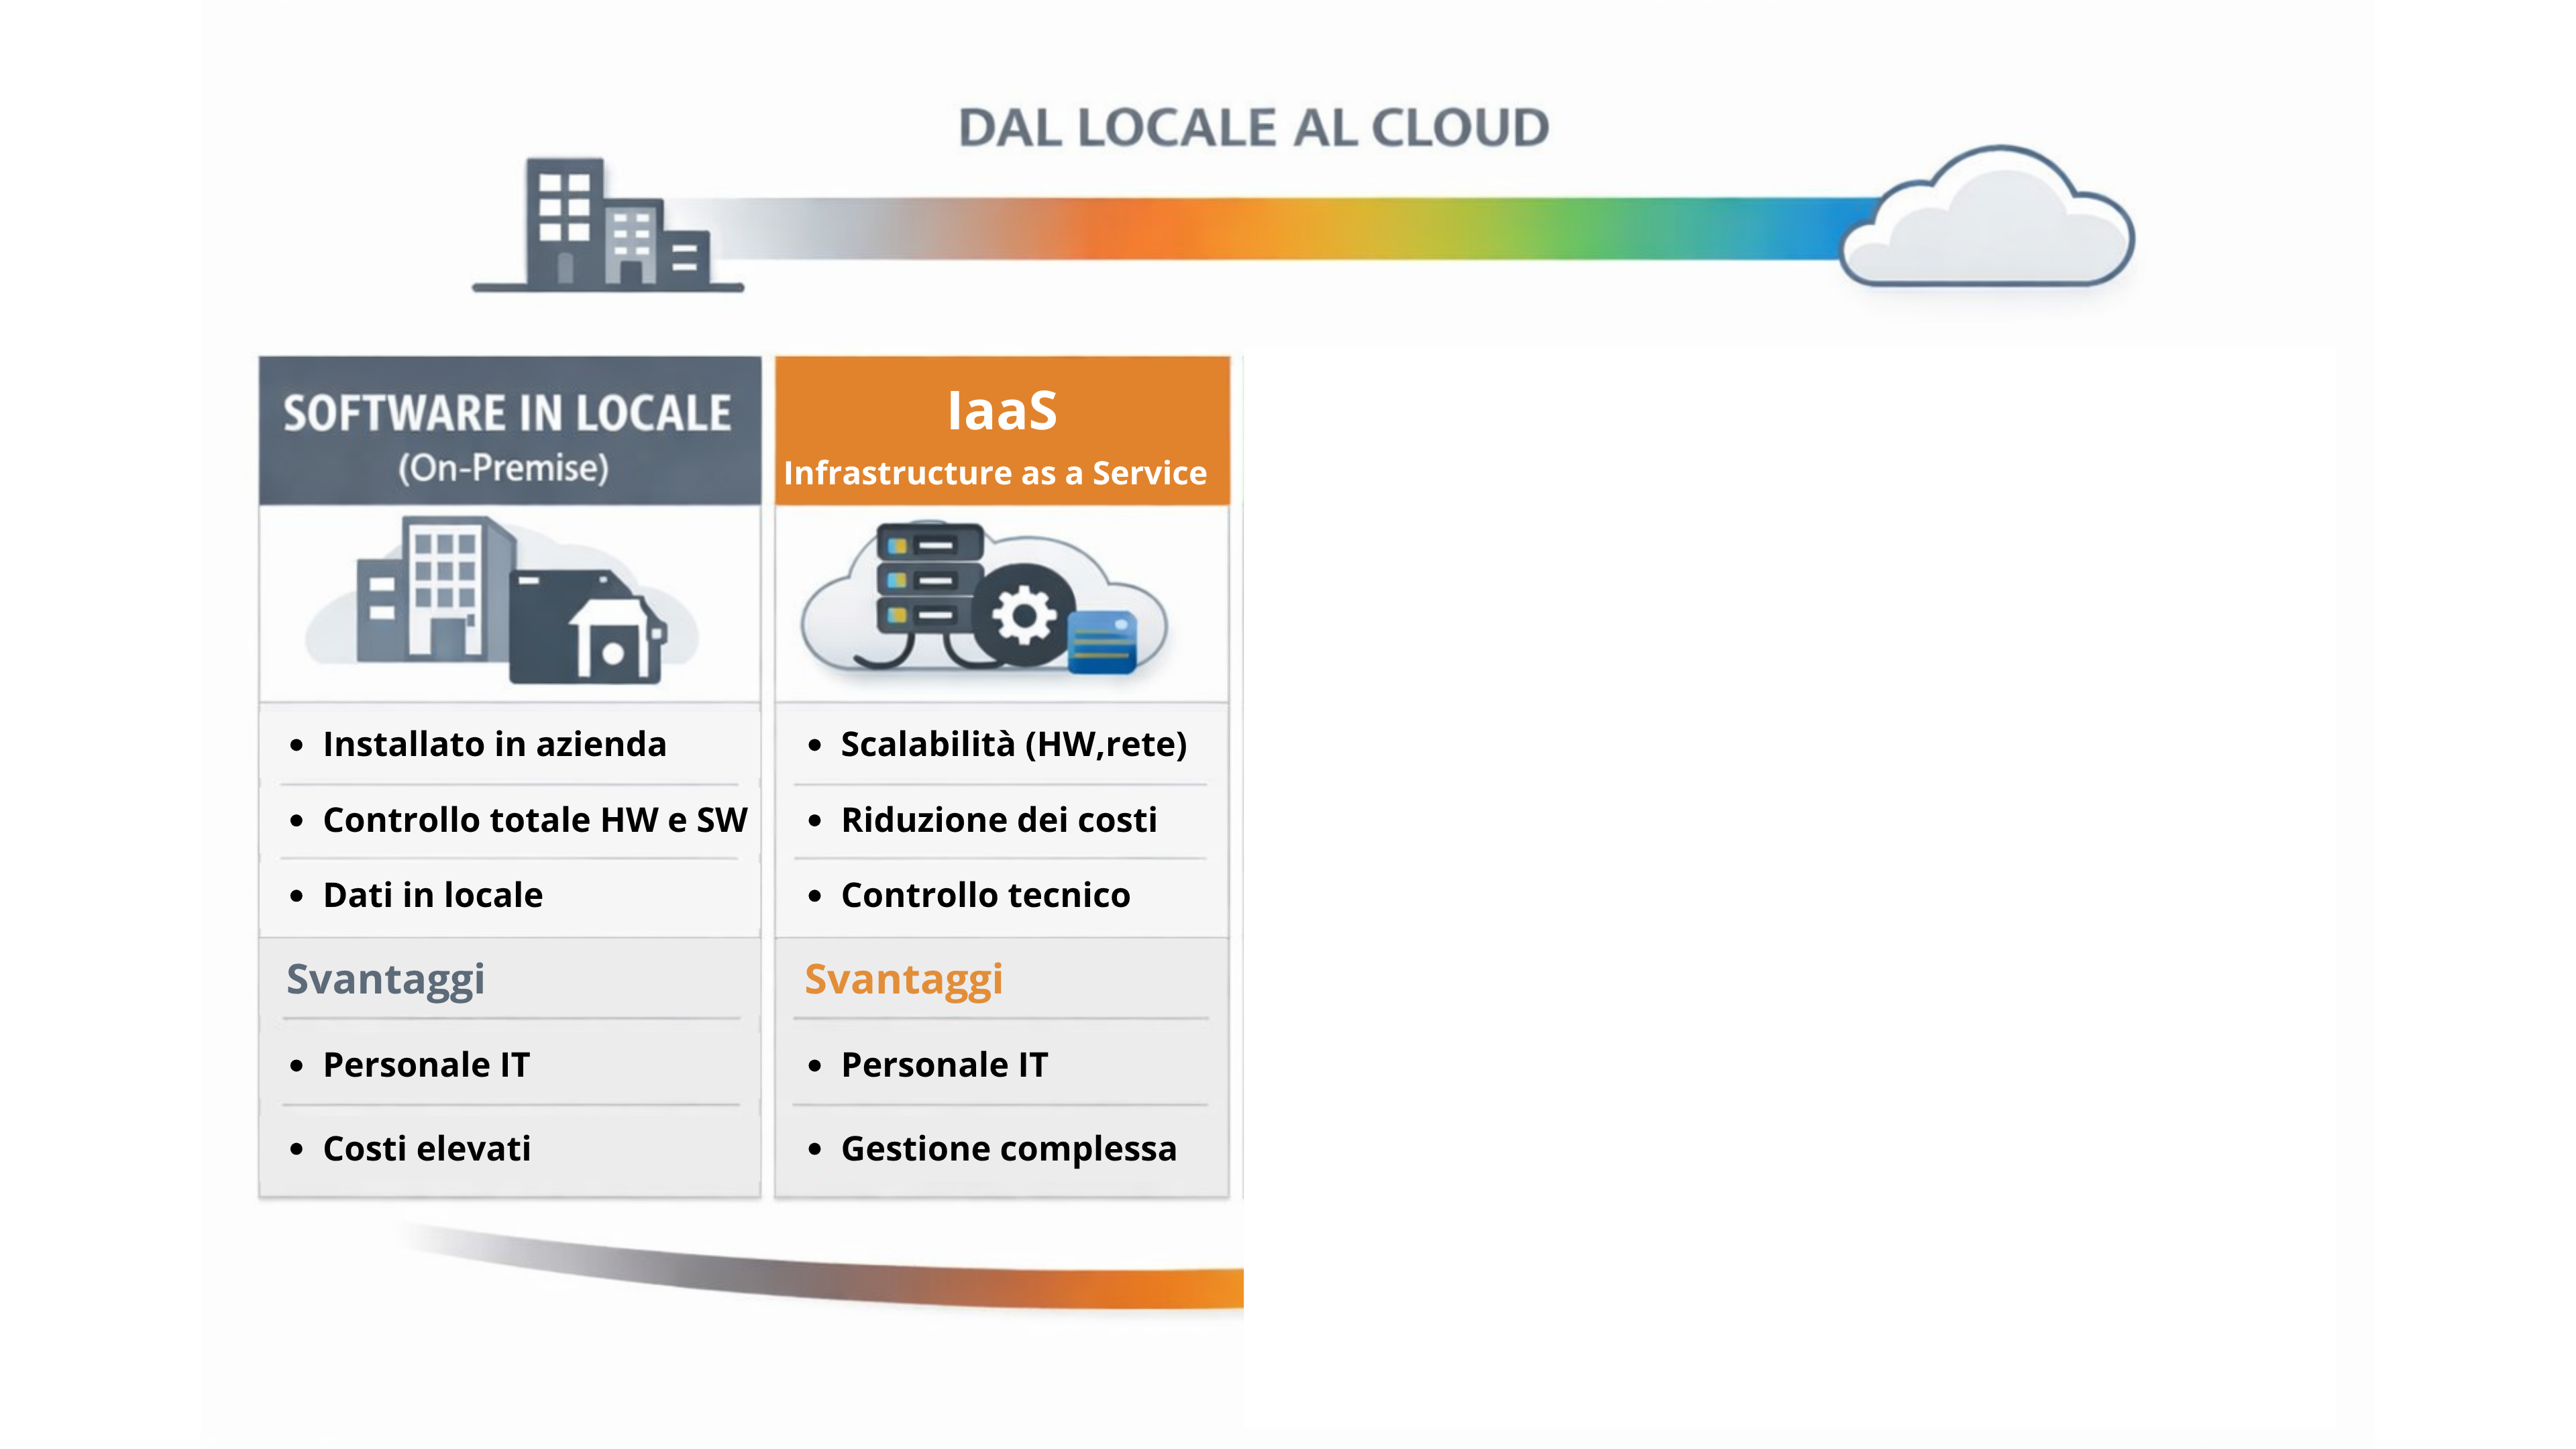
\includegraphics[width=\linewidth]{confronto3.png}
        \caption{{creata con \href{https://copilot.microsoft.com/}{Copilot}} e modificata con \href{https://www.canva.com/}{Canva}}
    \end{figure}}
    \only<4 | handout:3>{\begin{figure}
        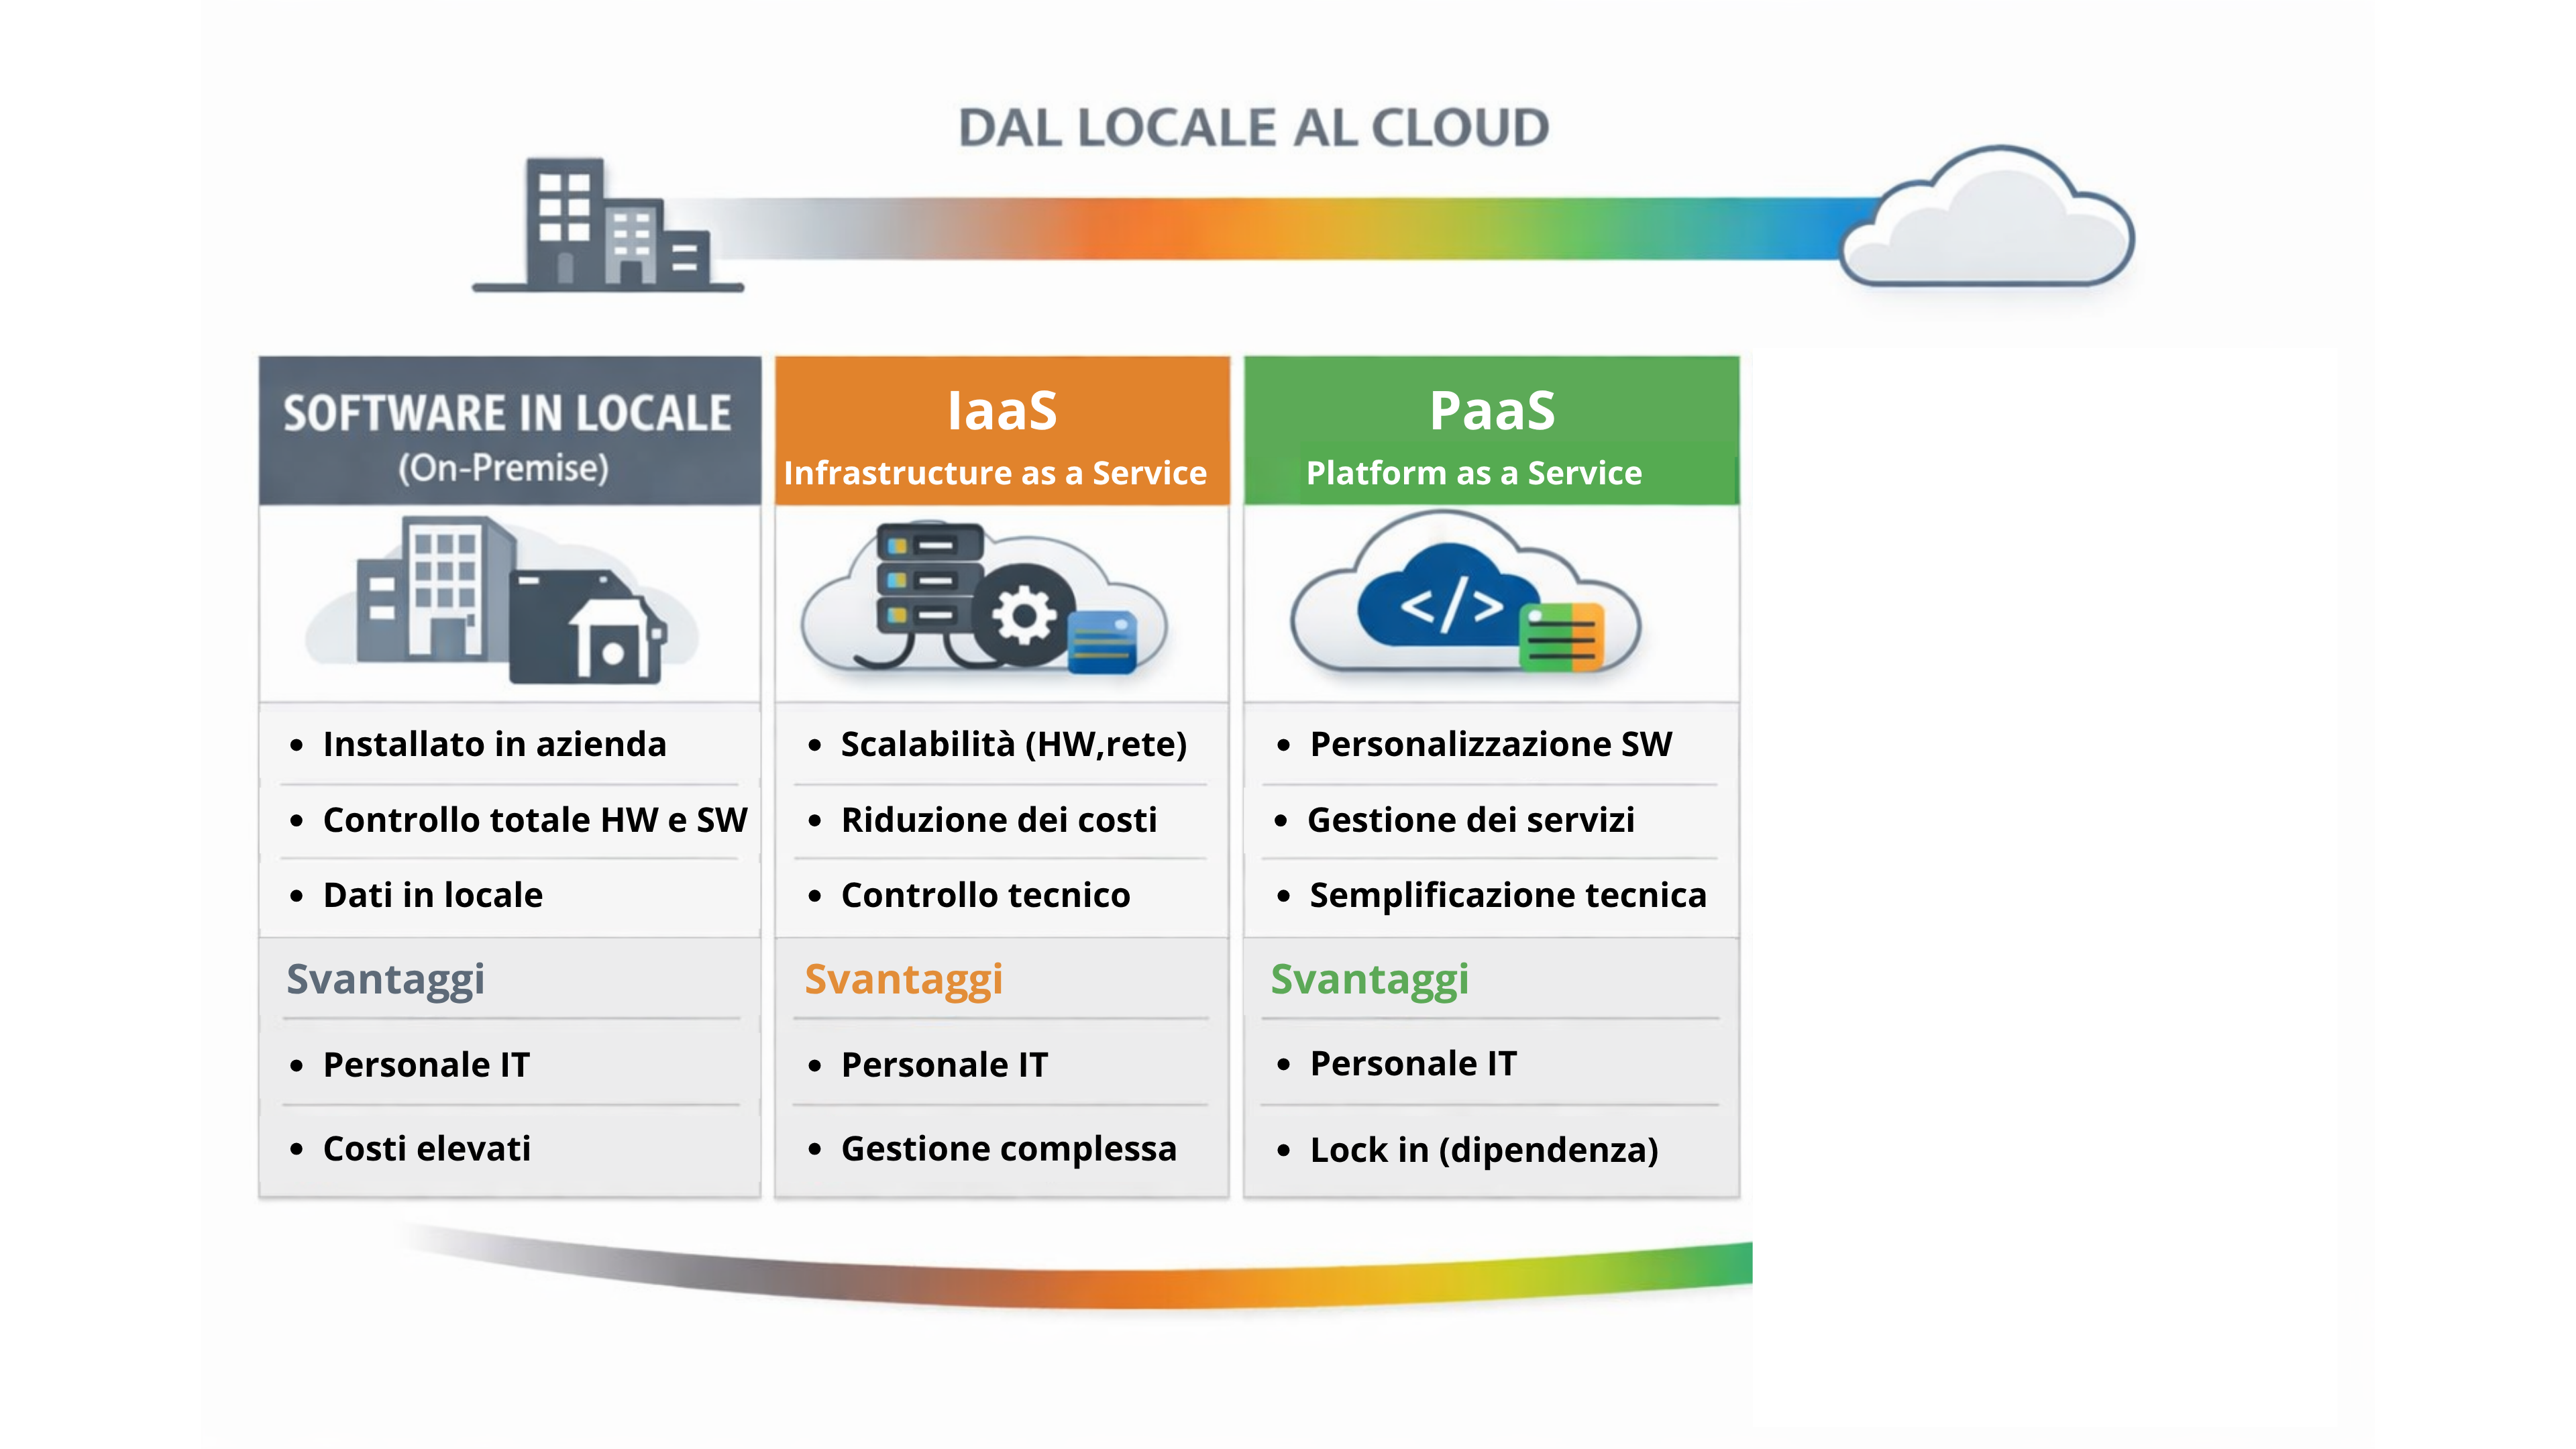
\includegraphics[width=\linewidth]{confronto4.png}
        \caption{{creata con \href{https://copilot.microsoft.com/}{Copilot}} e modificata con \href{https://www.canva.com/}{Canva}}
    \end{figure}}
    \only<5 | handout:3>{\begin{figure}
        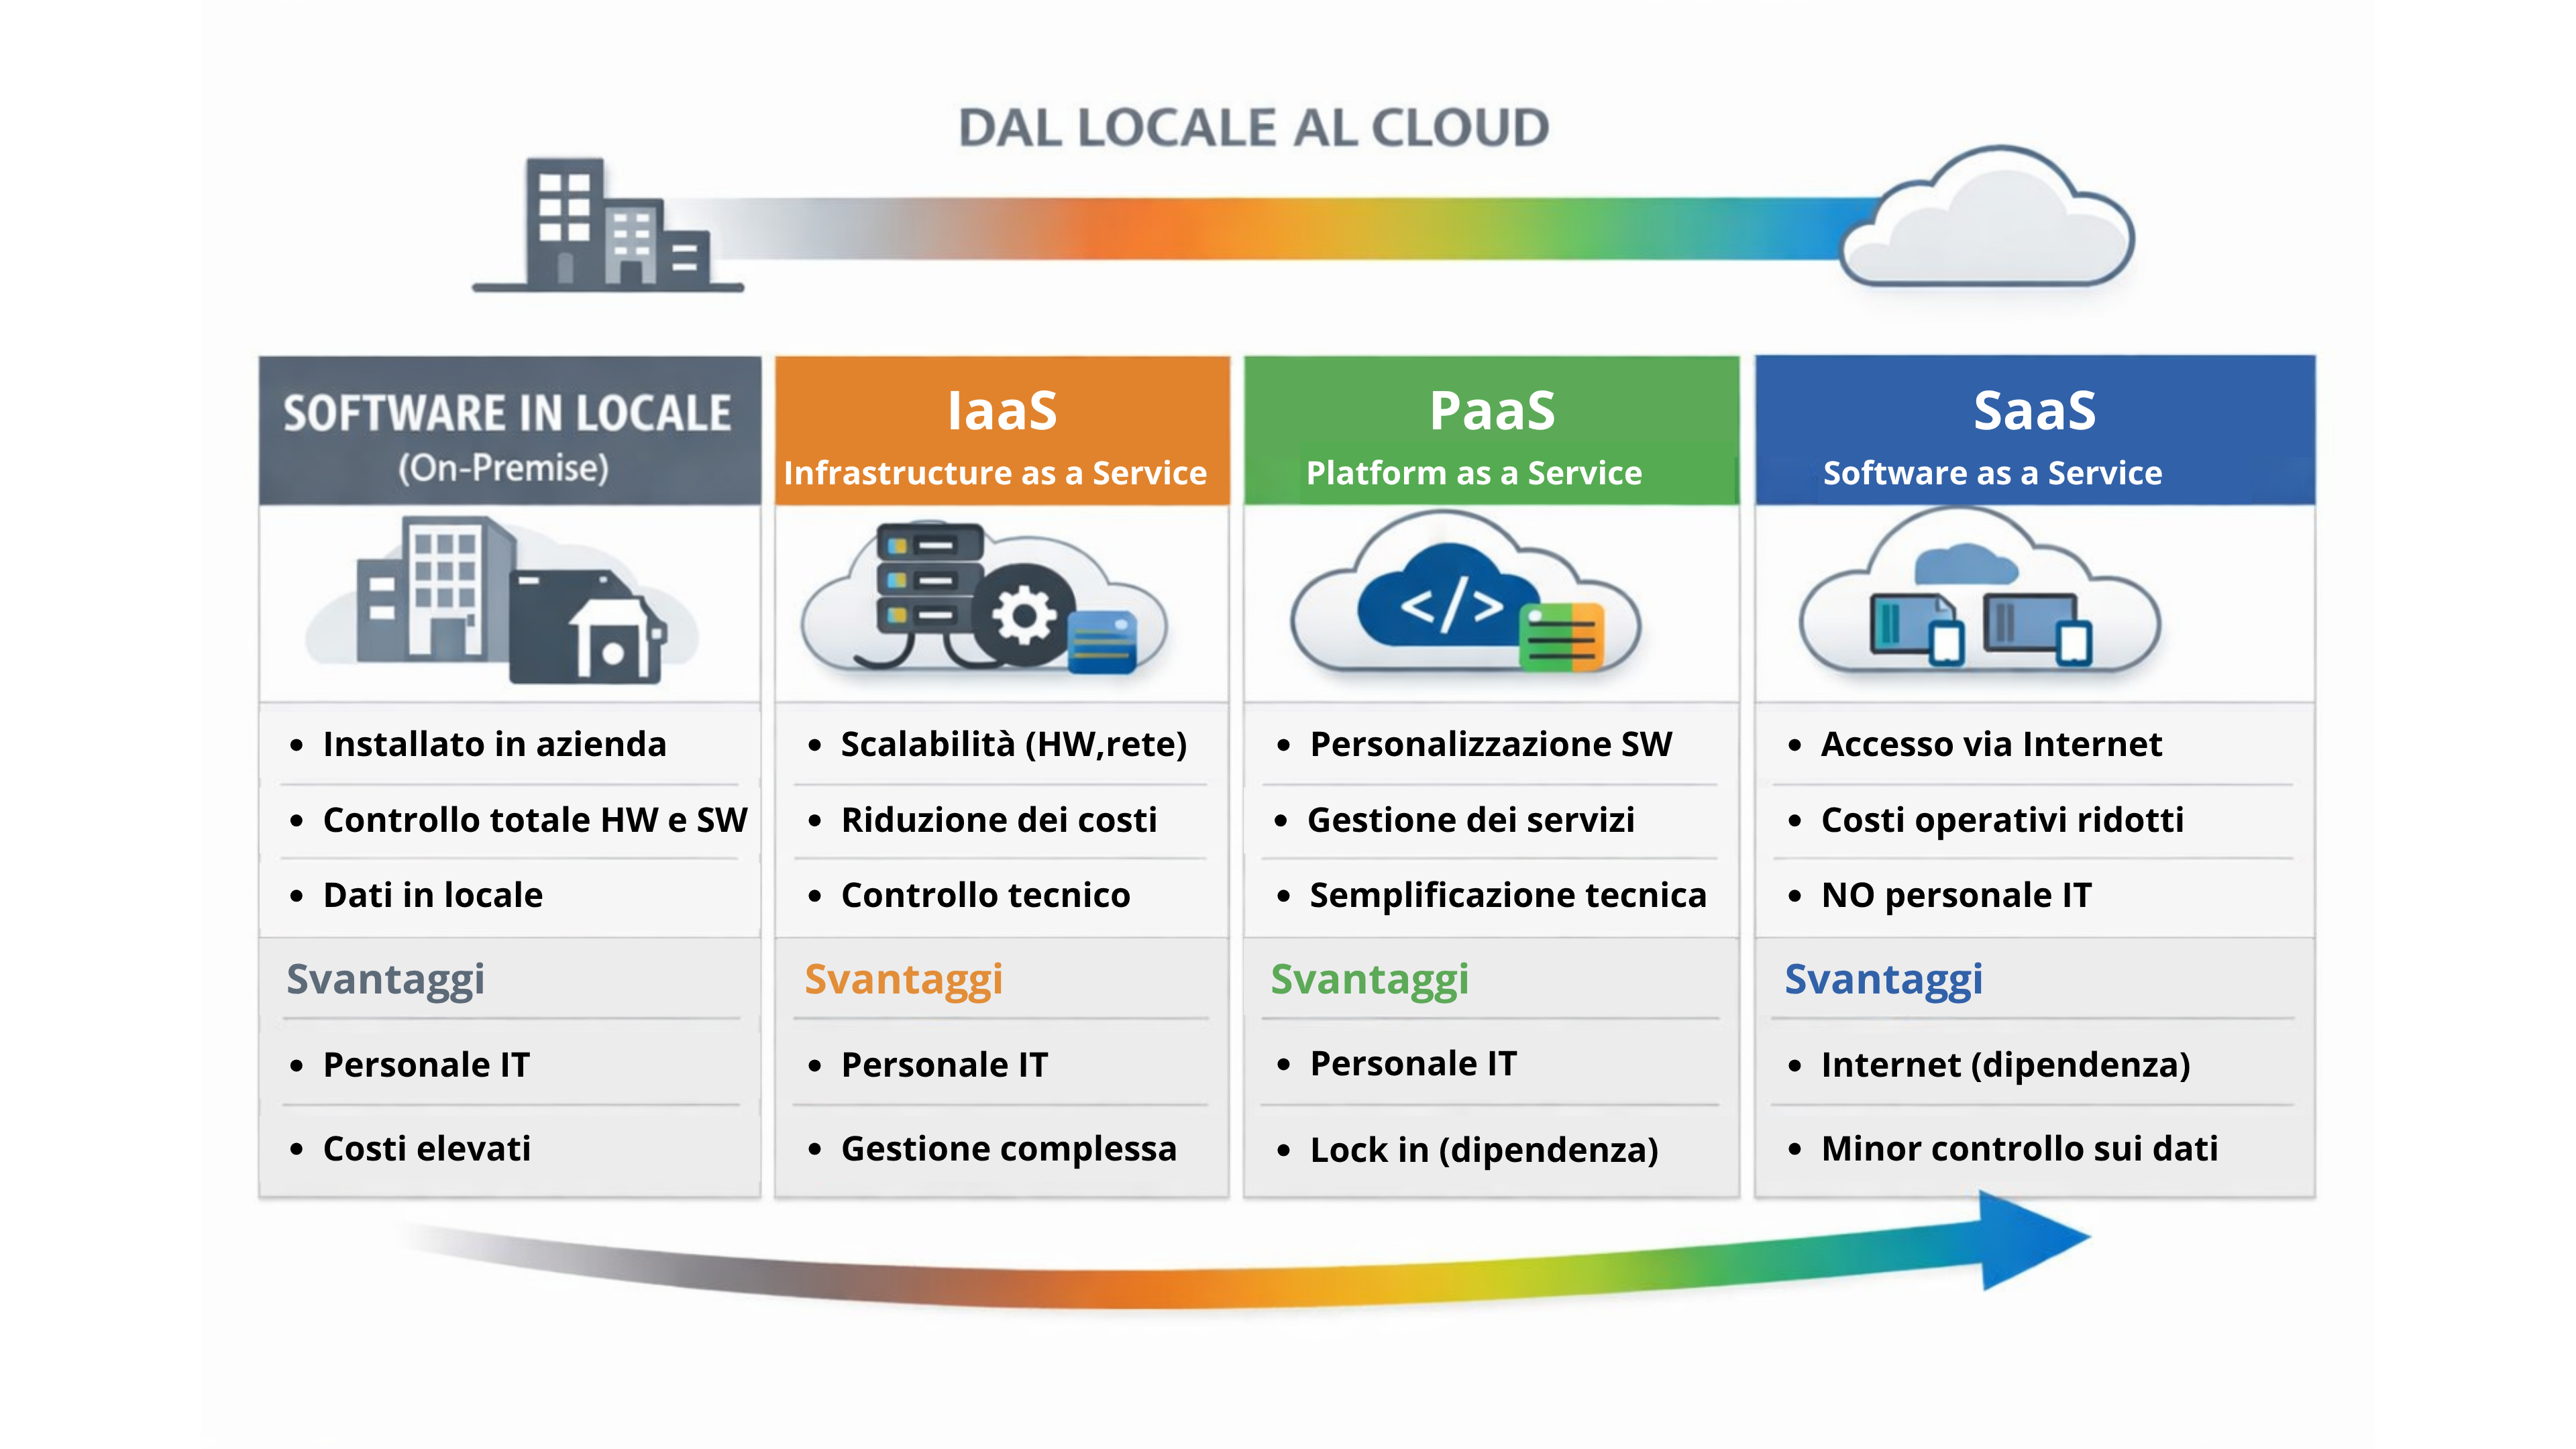
\includegraphics[width=\linewidth]{confronto5.png}
        \caption{{creata con \href{https://copilot.microsoft.com/}{Copilot}} e modificata con \href{https://www.canva.com/}{Canva}}
    \end{figure}}
    \only<6 | handout:3>{\begin{figure}
        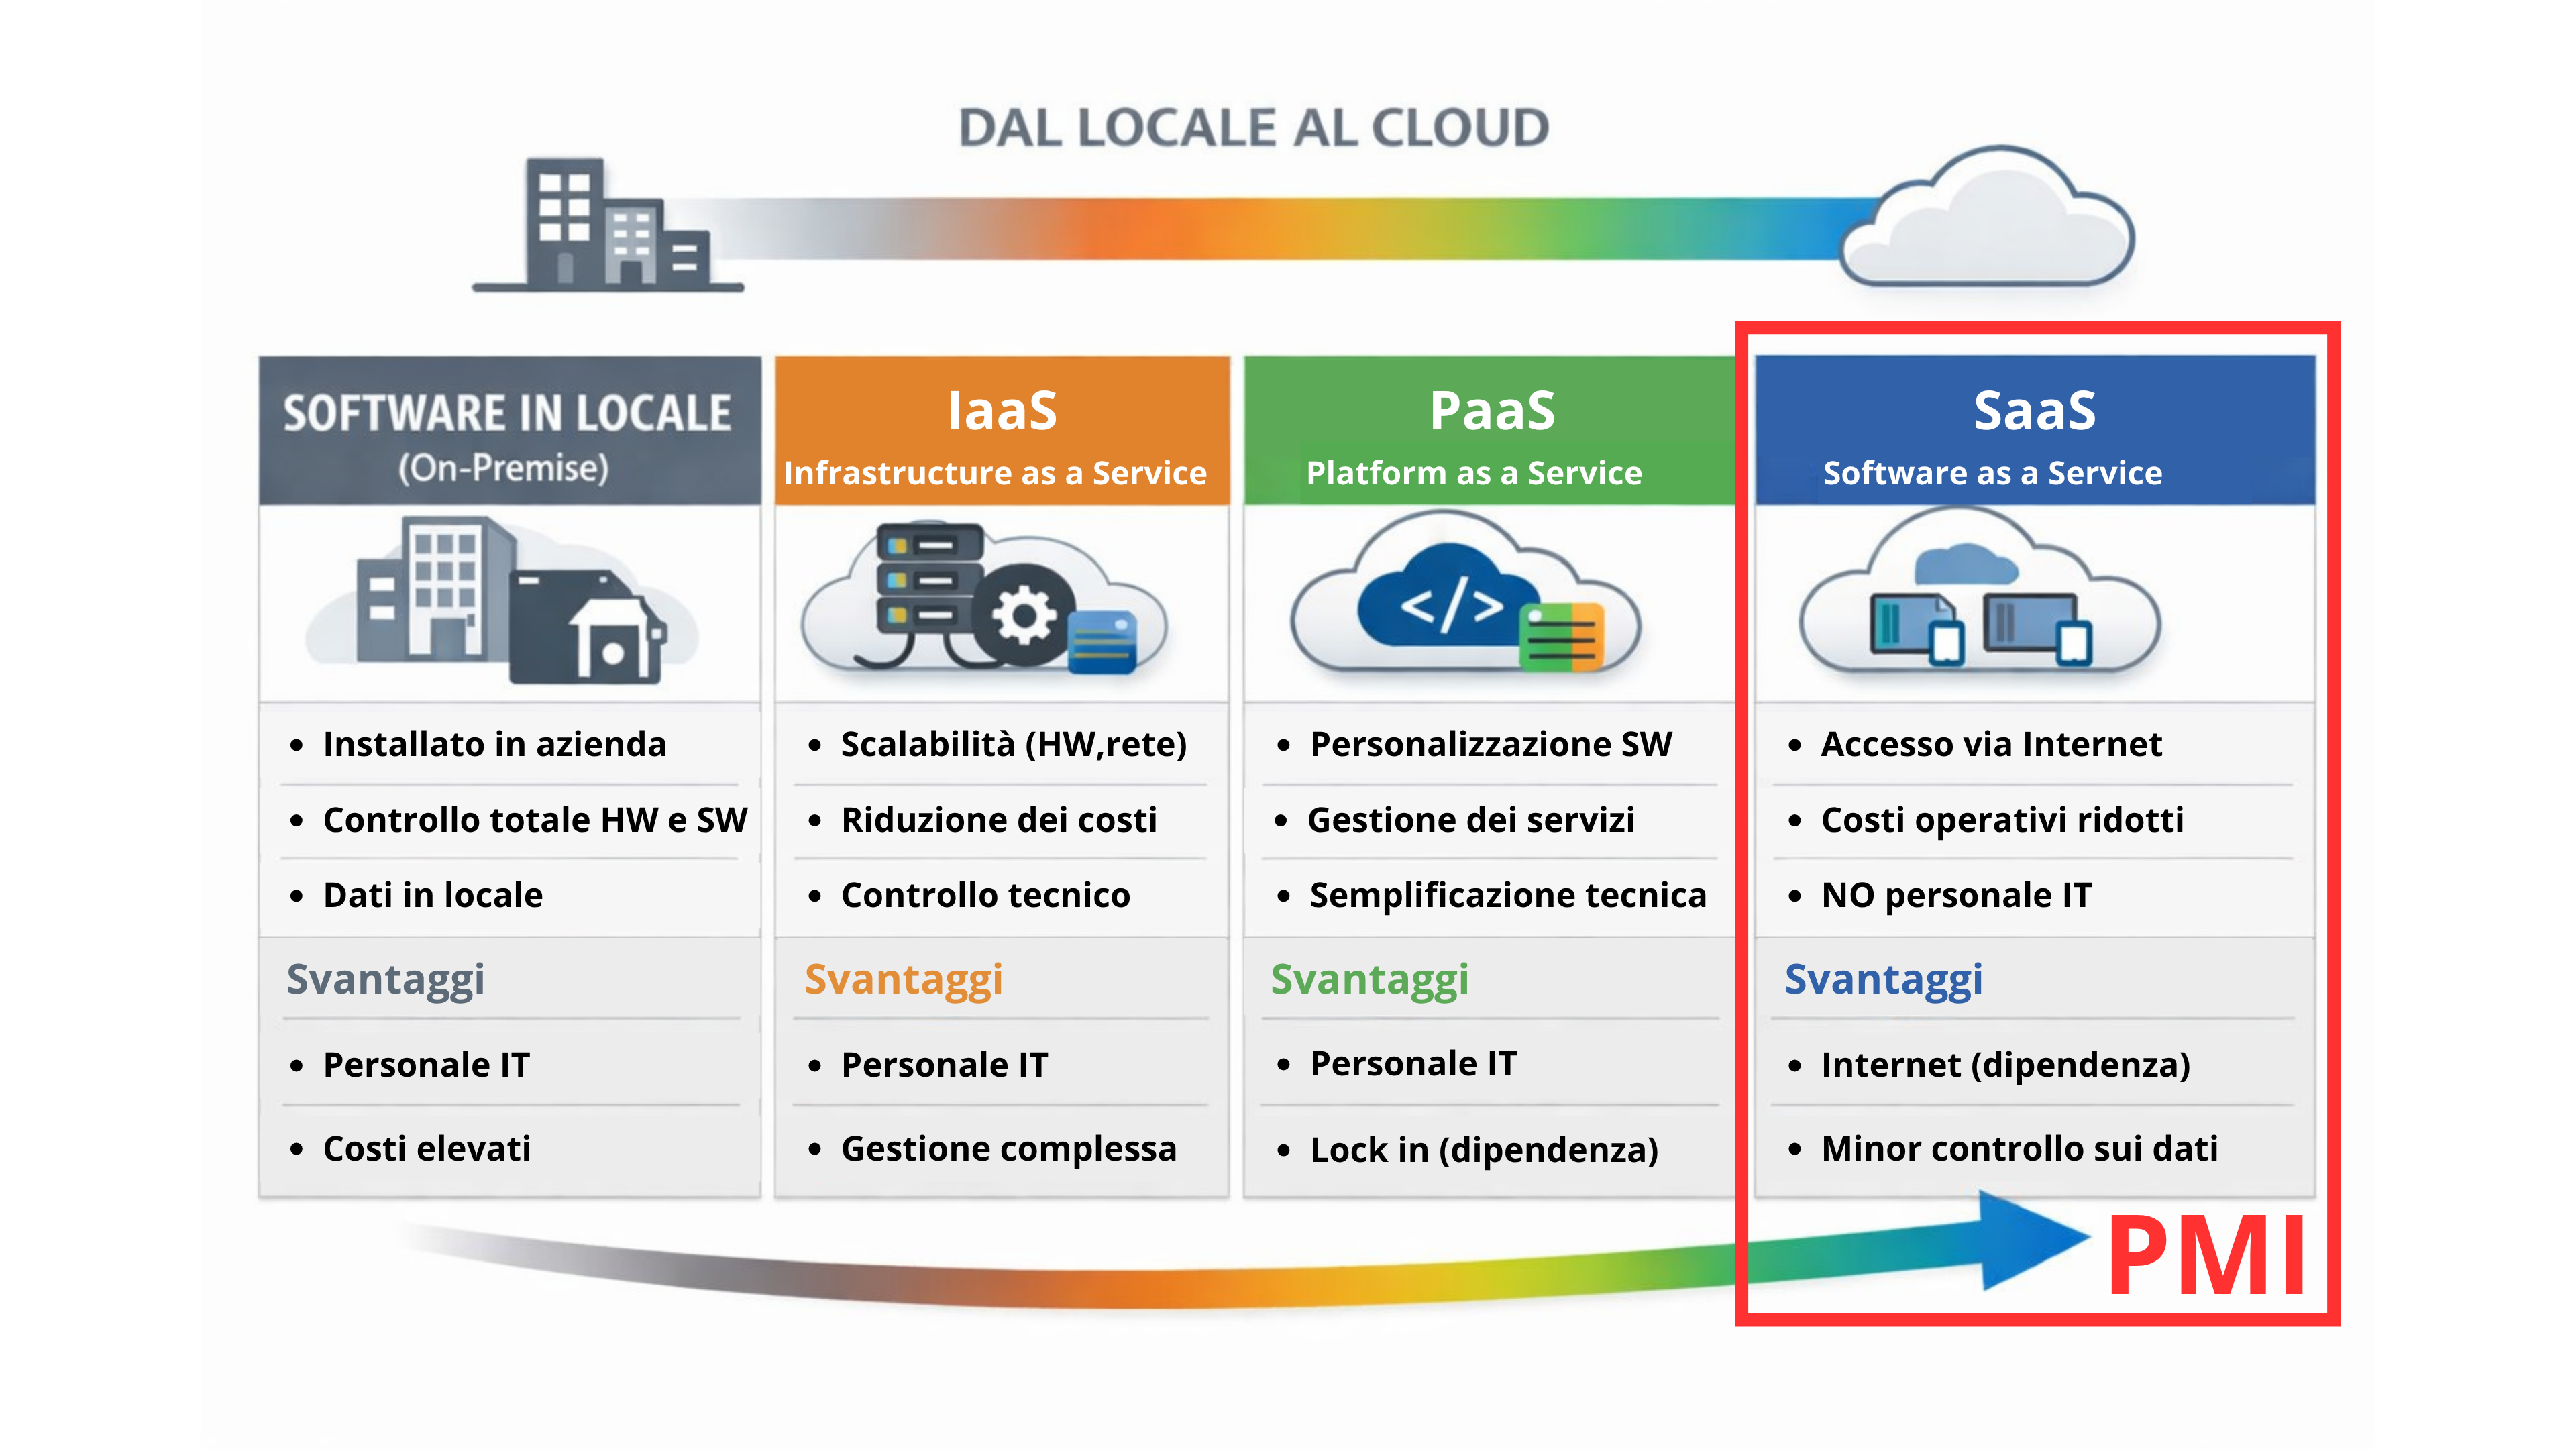
\includegraphics[width=\linewidth]{confronto6.png}
        \caption{{creata con \href{https://copilot.microsoft.com/}{Copilot}} e modificata con \href{https://www.canva.com/}{Canva}}
    \end{figure}}
\end{frame}

\begin{frame}{Quale SaaS scegliere?}
    \begin{alertblock}{CRITRI DI SCELTA}
        \begin{minipage}{0.98\linewidth}
            \justifying
            Non c'è una risposta univoca alla domanda su quale SaaS scegliere, poiché la scelta dipende 
            da molteplici fattori specifici dell'azienda, tuttavia, è possibile identificare alcuni 
            criteri chiave che possono guidare la decisione:
                \begin{itemize}
                    \pause
                    \item \textbf{Analisi delle esigenze aziendali}: funzionalità e processi da supportare;
                    \pause
                    \item \textbf{Valutazione dei costi}: valutare il modello di pricing e i costi nascosti.
                    \pause
                    \item \textbf{Scalabilità e flessibilità}: adattabilità a eventuali cambiamenti nelle esigenze.
                    \pause
                    \item \textbf{Supporto e assistenza}: supporto tecnico e qualità del servizio clienti.
                    \pause
                    \item \textbf{Sicurezza e conformità legali}: sicurezza e conformità alle normative (GDPR).
                    \pause
                    \item \textbf{Integrazione}: compatibilità con i sistemi e le applicazioni già in uso.
                    \pause
                    \item \textbf{Considerazioni etiche}: impatto ambientale e responsabilità sociale.
                    \pause
                    \item \textbf{Prova gratuita e demo}: testare il software prima di prendere una decisione.
                \end{itemize}
            \bigskip      
        \end{minipage}
    \end{alertblock}
\end{frame}

\begin{frame}{Learning by doing}
    \begin{figure}
        \href{https://www.odoo.com/it_IT}{
\includegraphics[width=.7\linewidth]{logo.png}}
        \bigskip
        \caption{{Link al sito della suite di software gestionali open-source \href{https://www.odoo.com/it_IT}{odoo}}}
    \end{figure}
\end{frame} 

\begin{frame}{Compito di realtà - Caso di studio}
    \begin{columns}
        \column{.6\textwidth}
            \begin{alertblock}{LEARNING BY DOING}
                \begin{minipage}{0.96\linewidth}
                    \justifying
                    \textbf{A coppie}, partendo da un \textbf{caso di studio reale}, mettetevi nei panni di un'
                    ipotetica PMI Italiana che ha intenzione di \textbf{utilizzare Odoo} come SaaS per gestire le 
                    proprie attività aziendali. \textbf{Configurate il software} in base alle esigenze specifiche 
                    dell'azienda, tenendo conto dei moduli più rilevanti per il settore di appartenenza e 
                    delle funzionalità necessarie \textbf{per ottimizzare i processi aziendali}. Compilate infine 
                    un \textbf{report} in cui spiegate le scelte effettuate e come Odoo può contribuire a 
                    \textbf{migliorare l'efficienza e la gestione dell'azienda}.
                    \bigskip
                \end{minipage}
            \end{alertblock}
        \column{.4\textwidth}
            \begin{figure}
                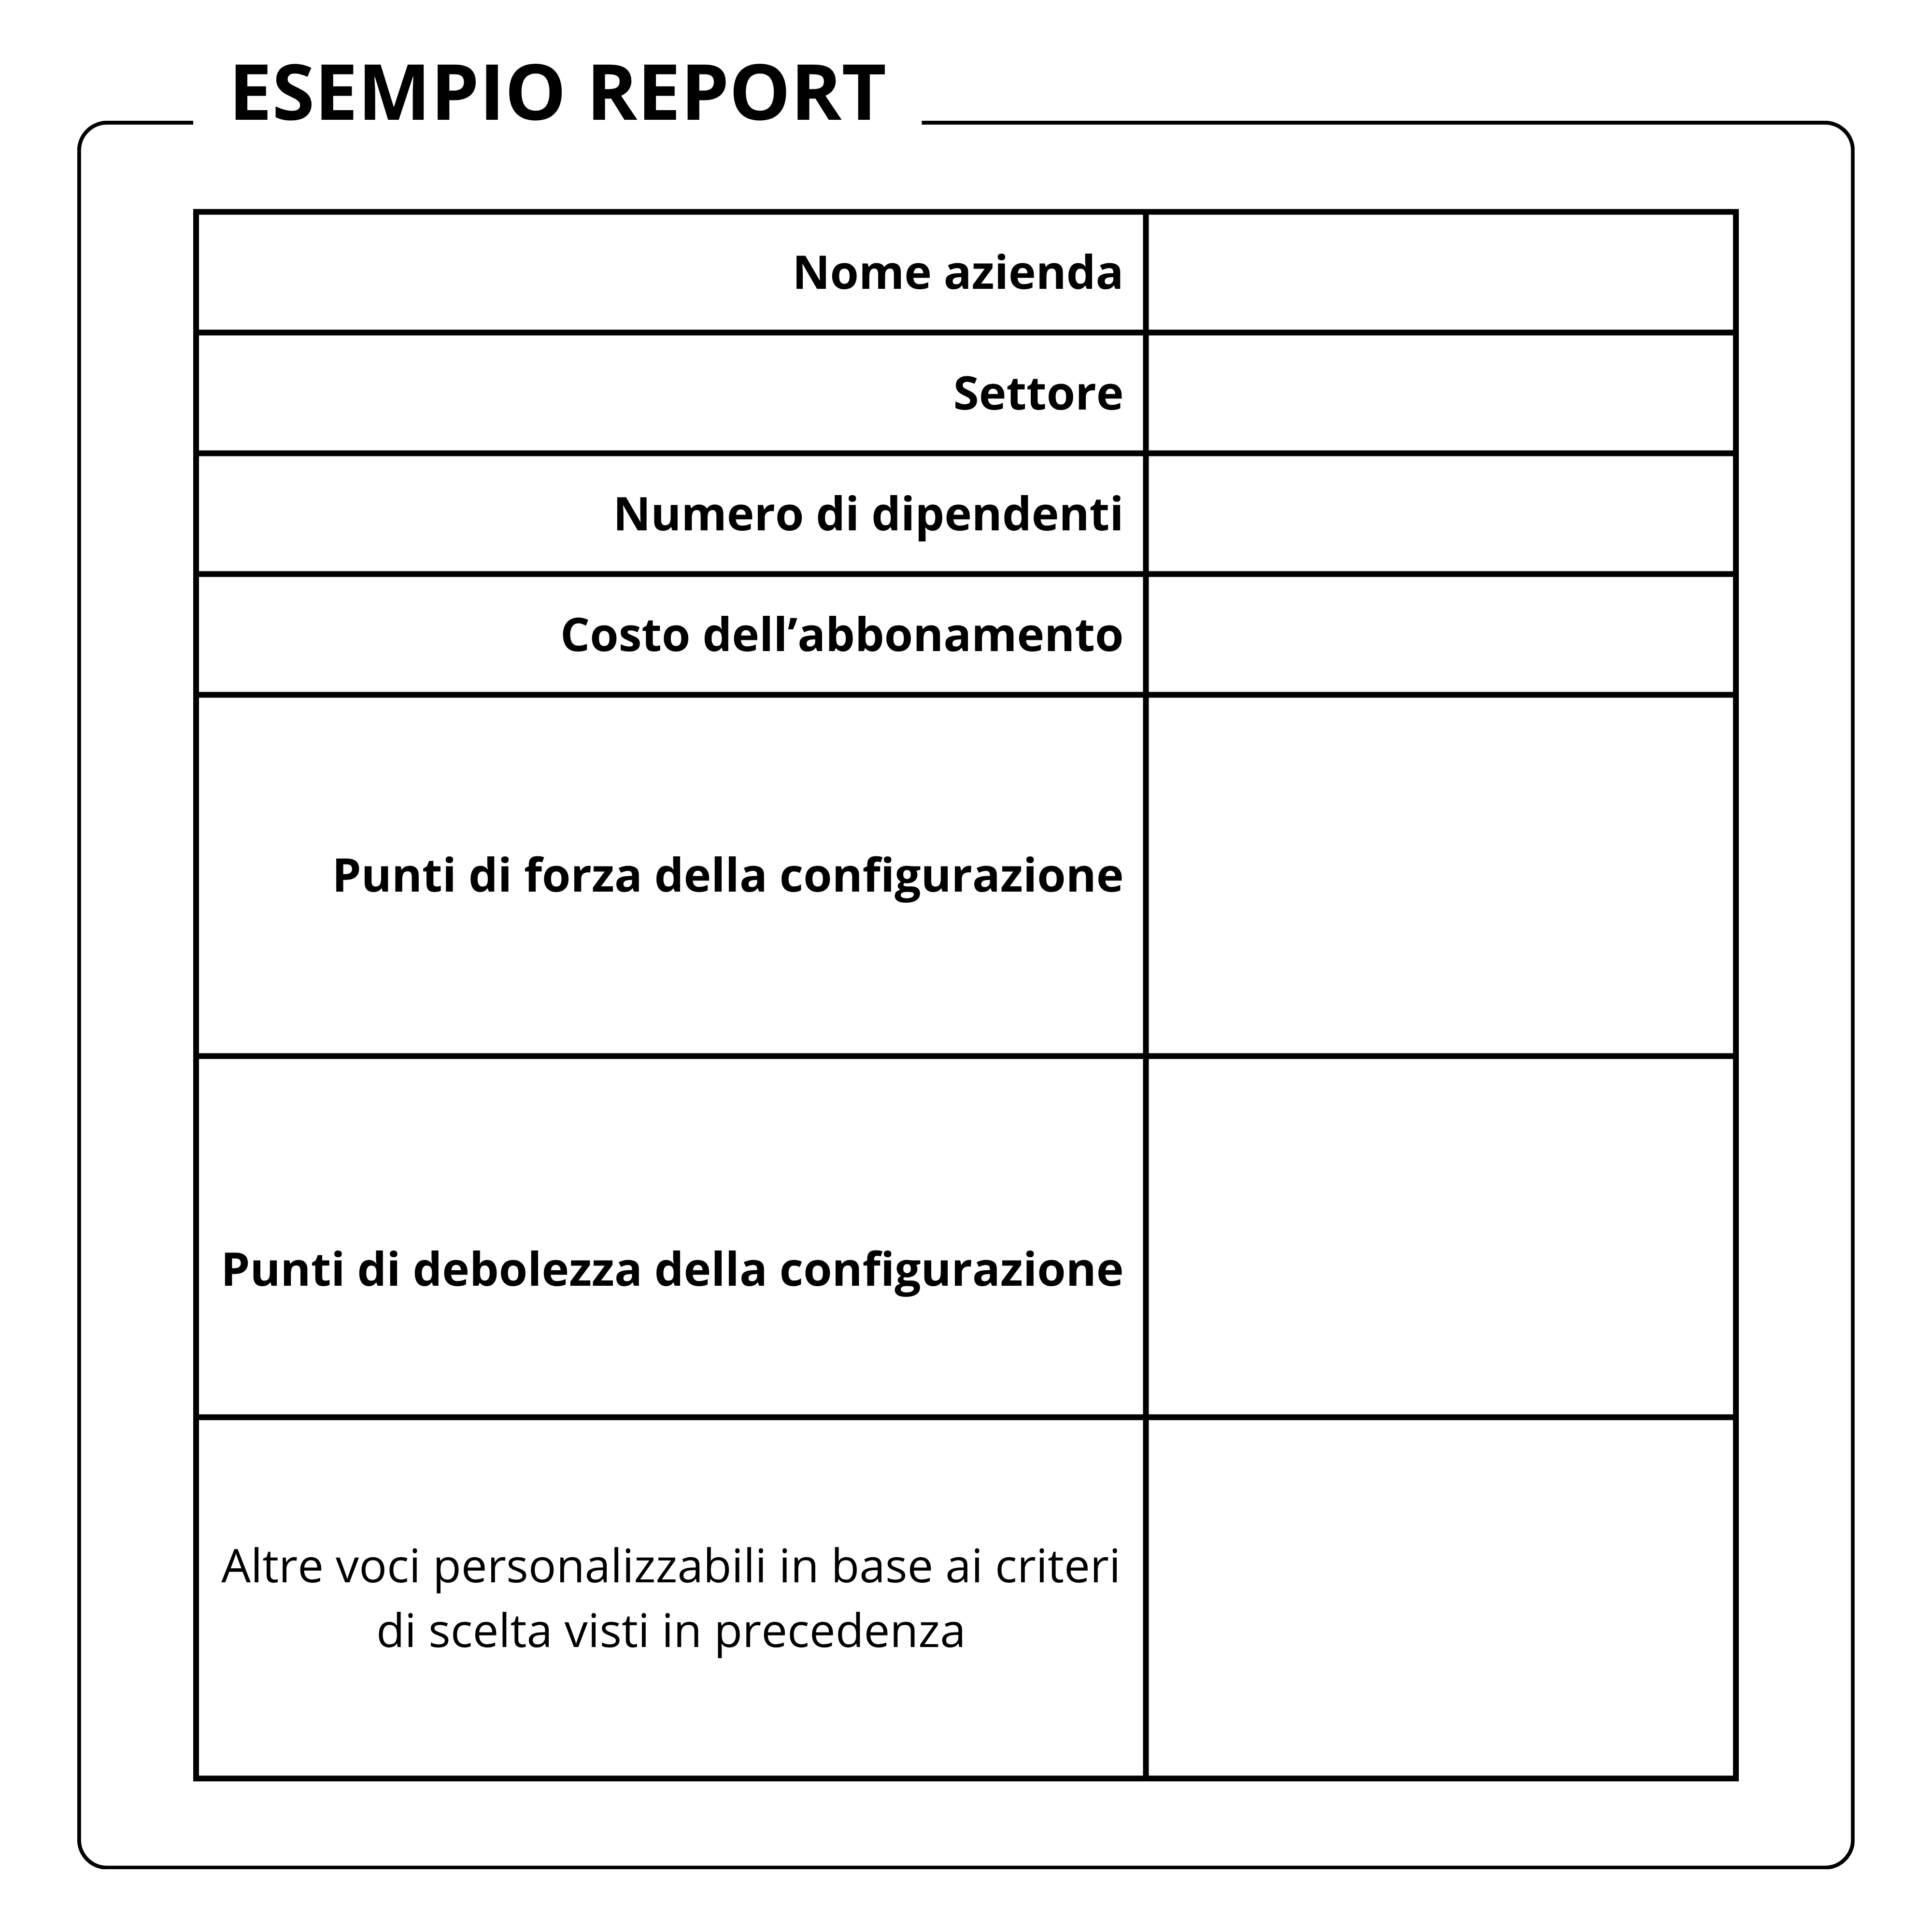
\includegraphics[width=\linewidth]{report.png}
                \caption{{creata con \href{www.canva.com}{Canva}}}
            \end{figure}
    \end{columns}
\end{frame}
\end{document}